\documentclass[conference]{IEEEtran}


%
% --- inline annotations
%
\newcommand{\red}[1]{{\color{red}#1}}
\newcommand{\todo}[1]{{\color{red}#1}}
\newcommand{\TODO}[1]{\textbf{\color{red}[TODO: #1]}}
% --- disable by uncommenting  
% \renewcommand{\TODO}[1]{}
% \renewcommand{\todo}[1]{#1}



\newcommand{\VLM}{LVLM\xspace} 
\newcommand{\ours}{PeKit\xspace}
\newcommand{\yollava}{Yo’LLaVA\xspace}

\newcommand{\thisismy}{This-Is-My-Img\xspace}
\newcommand{\myparagraph}[1]{\noindent\textbf{#1}}
\newcommand{\vdoro}[1]{{\color[rgb]{0.4, 0.18, 0.78} {[V] #1}}}
% --- disable by uncommenting  
% \renewcommand{\TODO}[1]{}
% \renewcommand{\todo}[1]{#1}
\usepackage{slashbox}
% Vectors
\newcommand{\bB}{\mathcal{B}}
\newcommand{\bw}{\mathbf{w}}
\newcommand{\bs}{\mathbf{s}}
\newcommand{\bo}{\mathbf{o}}
\newcommand{\bn}{\mathbf{n}}
\newcommand{\bc}{\mathbf{c}}
\newcommand{\bp}{\mathbf{p}}
\newcommand{\bS}{\mathbf{S}}
\newcommand{\bk}{\mathbf{k}}
\newcommand{\bmu}{\boldsymbol{\mu}}
\newcommand{\bx}{\mathbf{x}}
\newcommand{\bg}{\mathbf{g}}
\newcommand{\be}{\mathbf{e}}
\newcommand{\bX}{\mathbf{X}}
\newcommand{\by}{\mathbf{y}}
\newcommand{\bv}{\mathbf{v}}
\newcommand{\bz}{\mathbf{z}}
\newcommand{\bq}{\mathbf{q}}
\newcommand{\bff}{\mathbf{f}}
\newcommand{\bu}{\mathbf{u}}
\newcommand{\bh}{\mathbf{h}}
\newcommand{\bb}{\mathbf{b}}

\newcommand{\rone}{\textcolor{green}{R1}}
\newcommand{\rtwo}{\textcolor{orange}{R2}}
\newcommand{\rthree}{\textcolor{red}{R3}}
\usepackage{amsmath}
%\usepackage{arydshln}
\DeclareMathOperator{\similarity}{sim}
\DeclareMathOperator{\AvgPool}{AvgPool}

\newcommand{\argmax}{\mathop{\mathrm{argmax}}}     



\def\BibTeX{{\rm B\kern-.05em{\sc i\kern-.025em b}\kern-.08em
    T\kern-.1667em\lower.7ex\hbox{E}\kern-.125emX}}

% Ensure letter paper
\pdfpagewidth=8.5in
\pdfpageheight=11in


\newcommand{\hpcayear}{2025}
%%%%%%%%%%%%%%%%%%%%%%%%%%%%%%%%%%%%%%%%
%%%%%%%%%%%%%% -- UPDATE -- %%%%%%%%%%%%%%%
\newcommand{\hpcasubmissionnumber}{1724}


\pagenumbering{arabic}

%%%%%%%%%%%---SETME-----%%%%%%%%%%%%%
% \title{Giant: Accelerating LLMs through Mathematically Adaptive Numeric Types Quantization}
\title{M-ANT: Efficient Low-bit Group Quantization for LLMs via Mathematically Adaptive Numerical Type 
\thanks{\IEEEauthorrefmark{1} Jingwen Leng is corresponding authors of this paper.}
}

%%%%%%%%%%%%%%%%%%%%%%%%%%%%%%%%%%%%%
%%%%%%%%%% -- DO NOT MODIFY -- %%%%%%%%%%
%%%%%%%%%%%%%%%%%%%%%%%%%%%%%%%%%%%%%

% \author{
%   \ifdefined\hpcacameraready
%     \IEEEauthorblockN{\hpcaauthors{}}
%       \IEEEauthorblockA{
%         \hpcaaffiliation{} \\
%         \hpcaemail{}
%       }
%   \else
%     \IEEEauthorblockN{\normalsize{HPCA \hpcayear{} Submission
%       \textbf{\#\hpcasubmissionnumber{}}} \\
%       \IEEEauthorblockA{
%         Confidential Draft \\
%         Do NOT Distribute!!
%       }
%     }
%   \fi 
% }
\author{
  \IEEEauthorblockN{
    Weiming Hu$^{1, 2}$,
    Haoyan Zhang$^{1, 2}$,
    Cong Guo$^3$, 
    Yu Feng$^{1}$,
    Renyang Guan$^{1, 2}$,
    Zhendong Hua$^{1}$,
    Zihan Liu$^{1, 2}$, \\
    Yue Guan$^{1, 2}$, 
    Minyi Guo$^{1, 2}$,
    Jingwen Leng$^{1, 2,}$\IEEEauthorrefmark{1}
  }
  \IEEEauthorblockA{
    $^1$Shanghai Jiao Tong University, $^2$Shanghai Qi Zhi Institute, $^3$Duke University \\
    \{weiminghu, h.y.zhang-zdy, y-feng, guanrenyang, jackeyhua, altair.liu, bonboru\}@sjtu.edu.cn, \\ \{guo-my, leng-jw\}@cs.sjtu.edu.cn, cong.guo@duke.edu
  }

}

\def\hpcacameraready{} % Uncomment to build camera-ready version
\newcommand{\hpcapubid}{0000--0000/00\$00.00}

% Heading and footer for title page
\fancypagestyle{camerareadyfirstpage}{%
  \fancyhead{}
  \renewcommand{\headrulewidth}{0pt}
  \fancyhead[C]{
    \ifdefined\aeopen
    \parbox[][12mm][t]{13.5cm}{\hpcayear{} IEEE International Symposium on High-Performance Computer Architecture (HPCA)}    
    \else
      \ifdefined\aereviewed
      \parbox[][12mm][t]{13.5cm}{\hpcayear{} IEEE International Symposium on High-Performance Computer Architecture (HPCA)}
      \else
      \ifdefined\aereproduced
      \parbox[][12mm][t]{13.5cm}{\hpcayear{} IEEE International Symposium on High-Performance Computer Architecture (HPCA)}
      \else
      \parbox[][0mm][t]{13.5cm}{\hpcayear{} IEEE International Symposium on High-Performance Computer Architecture (HPCA)}
    \fi 
    \fi 
    \fi 
    \ifdefined\aeopen 
      \includegraphics[width=12mm,height=12mm]{ae-badges/open-research-objects.pdf}
    \fi 
    \ifdefined\aereviewed
      \includegraphics[width=12mm,height=12mm]{ae-badges/research-objects-reviewed.pdf}
    \fi 
    \ifdefined\aereproduced
      \includegraphics[width=12mm,height=12mm]{ae-badges/results-reproduced.pdf}
    \fi
  }
  %\fancyfoot[L]{\hpcapubid{} \copyright \hpcayear{} IEEE}
  \fancyfoot[C]{}
}
% Heading and footer for remaining pages
\fancyhead{}
\renewcommand{\headrulewidth}{0pt}
%\fancyhead[C]{\hpcayear{} IEEE International Symposium on
% High-Performance Computer Architecture (HPCA)}



\begin{document}

% \documentclass[10pt,twocolumn,letterpaper]{article}
\usepackage[rebuttal]{cvpr}

% Include other packages here, before hyperref.
\usepackage{graphicx}
\usepackage{amsmath}
\usepackage{amssymb}
\usepackage{booktabs}
\usepackage{color}
\usepackage{colortbl}
% \usepackage{ulem}
% \useunder{\uline}{\ul}{}
% Import additional packages in the preamble file, before hyperref
%
% --- inline annotations
%
\newcommand{\red}[1]{{\color{red}#1}}
\newcommand{\todo}[1]{{\color{red}#1}}
\newcommand{\TODO}[1]{\textbf{\color{red}[TODO: #1]}}
% --- disable by uncommenting  
% \renewcommand{\TODO}[1]{}
% \renewcommand{\todo}[1]{#1}



\newcommand{\VLM}{LVLM\xspace} 
\newcommand{\ours}{PeKit\xspace}
\newcommand{\yollava}{Yo’LLaVA\xspace}

\newcommand{\thisismy}{This-Is-My-Img\xspace}
\newcommand{\myparagraph}[1]{\noindent\textbf{#1}}
\newcommand{\vdoro}[1]{{\color[rgb]{0.4, 0.18, 0.78} {[V] #1}}}
% --- disable by uncommenting  
% \renewcommand{\TODO}[1]{}
% \renewcommand{\todo}[1]{#1}
\usepackage{slashbox}
% Vectors
\newcommand{\bB}{\mathcal{B}}
\newcommand{\bw}{\mathbf{w}}
\newcommand{\bs}{\mathbf{s}}
\newcommand{\bo}{\mathbf{o}}
\newcommand{\bn}{\mathbf{n}}
\newcommand{\bc}{\mathbf{c}}
\newcommand{\bp}{\mathbf{p}}
\newcommand{\bS}{\mathbf{S}}
\newcommand{\bk}{\mathbf{k}}
\newcommand{\bmu}{\boldsymbol{\mu}}
\newcommand{\bx}{\mathbf{x}}
\newcommand{\bg}{\mathbf{g}}
\newcommand{\be}{\mathbf{e}}
\newcommand{\bX}{\mathbf{X}}
\newcommand{\by}{\mathbf{y}}
\newcommand{\bv}{\mathbf{v}}
\newcommand{\bz}{\mathbf{z}}
\newcommand{\bq}{\mathbf{q}}
\newcommand{\bff}{\mathbf{f}}
\newcommand{\bu}{\mathbf{u}}
\newcommand{\bh}{\mathbf{h}}
\newcommand{\bb}{\mathbf{b}}

\newcommand{\rone}{\textcolor{green}{R1}}
\newcommand{\rtwo}{\textcolor{orange}{R2}}
\newcommand{\rthree}{\textcolor{red}{R3}}
\usepackage{amsmath}
%\usepackage{arydshln}
\DeclareMathOperator{\similarity}{sim}
\DeclareMathOperator{\AvgPool}{AvgPool}

\newcommand{\argmax}{\mathop{\mathrm{argmax}}}     



% If you comment hyperref and then uncomment it, you should delete
% egpaper.aux before re-running latex.  (Or just hit 'q' on the first latex
% run, let it finish, and you should be clear).
\definecolor{cvprblue}{rgb}{0.21,0.49,0.74}
\definecolor{mygray}{gray}{.9}
\usepackage[pagebackref,breaklinks,colorlinks,citecolor=cvprblue]{hyperref}


\newcommand{\re}[2]{\textcolor{#1}{{\bf #2}}}

% Support for easy cross-referencing
\usepackage[capitalize]{cleveref}
\crefname{section}{Sec.}{Secs.}
\Crefname{section}{Section}{Sections}
\Crefname{table}{Table}{Tables}
\crefname{table}{Tab.}{Tabs.}

% If you wish to avoid re-using figure, table, and equation numbers from
% the main paper, please uncomment the following and change the numbers
% appropriately.
%\setcounter{figure}{2}
\setcounter{table}{0}
\renewcommand\thetable{Rb\arabic{table}}
%\setcounter{equation}{2}

% If you wish to avoid re-using reference numbers from the main paper,
% please uncomment the following and change the counter for `enumiv' to
% the number of references you have in the main paper (here, 6).
%\let\oldthebibliography=\thebibliography
%\let\oldendthebibliography=\endthebibliography
%\renewenvironment{thebibliography}[1]{%
%     \oldthebibliography{#1}%
%     \setcounter{enumiv}{6}%
%}{\oldendthebibliography}


%%%%%%%%% PAPER ID  - PLEASE UPDATE
\def\paperID{2514} % *** Enter the Paper ID here
\def\confName{CVPR}
\def\confYear{2025}

\begin{document}

%%%%%%%%% TITLE - PLEASE UPDATE
\title{Category-Level Object Pose Estimation via Causal Learning and Knowledge Distillation}  % **** Enter the paper title here

\maketitle
\thispagestyle{empty}
\appendix

%%%%%%%%% BODY TEXT - ENTER YOUR RESPONSE BELOW
% \section{Introduction}
% \re{red}{R1} \re{blue}{R2} \re{green}{R3}
\noindent
We appreciate reviewers for their valuable feedback, acknowledging the \emph{“clarity and novelty”} (\re{green}{rYxx@R3}) of our core idea, as well as the \emph{“detailed formulation provided”} (\re{blue}{qCQv@R2}). We are encouraged they recognize our approach \emph{“well-organized and easy to follow”} (\re{blue}{R2}, \re{green}{R3}), evaluated with \emph{“extensive experiments”} (\re{green}{R3}), and \emph{“achieving {\bf \emph{SOTA}} performance”} in multiple benchmarks (\re{red}{QHjZ@R1}, \re{blue}{R2}, \re{green}{R3}). We sincerely thank the reviewers for their diligent work and hope our response meets their approval.

\noindent
{\bf $\triangleright$ Responses to individual questions for each reviewer.}

\noindent
\re{red}{@R1 \#w1:} {\bf The Clarity of Paper.}  Thanks for your feedback! Key terms such as \emph{“confounders”} and \emph{“front-door path”} are formally introduced in Sec.3.2 (L201-214), and the causal modeling is illustrated in Fig.2. To improve clarity, we will further enhance the explanation of these key concepts by providing more concrete examples from the task domain and clarifying their roles in the methodology. Additionally, we will confirm that the causal modeling process is presented more intuitively to make it easier to follow.

\noindent
\re{red}{@R1 \#w2:} {\bf The Novelty of Method.} We appreciate your concerns. The key novelty and contribution of our work lies in integrating causal theoretical foundation [36, 37] into COPE models. As Reviewer 3 noted: \emph{“this idea is novel and not straightforward”}. To the best of our knowledge, we are the first to introduce causal modeling to enhance COPE models and achieve significant improvements. Therefore, our work is not simply a combination of existing methods, which involves careful exploration and design that addresses specific challenges mitigating confounding effects.


\noindent
\re{red}{@R1 \#w3:} {\bf Fairness of Comparison.} We would address your comment in two aspects: First, one of the contributions in our work is to explore how to better utilize 3D foundation models to enhance generalization, which is closely related to the overall design of our method, rather than introducing “extra knowledge” that benefits the comparison. Second, 3D foundation model only provides supervision during training, meaning it would not increase any computational burden during inference.
% as shown in \cref{tab:ablation_main} (\#1, \#2).
As for the comparison, we followed the domain consensus to report the metric accuracy.
In response to your suggestions, we have added more terms (\eg encoder type, inference latency) in \cref{tab:ablation_main} for comprehensive comparison. Due to space limitations, detailed comparisons and explanations will be included in revision.

\noindent
\re{blue}{@R2 \#w1:} {\bf Efficacy of Causal Learning.} In fact, as shown in Tab. \textcolor{red}{4}, introducing causal inference can already achieves SOTA results in the rigorous metric of 5°2\emph{cm}, 5°5\emph{cm} and 10°2\emph{cm}, surpassing the baseline by 2.7\%, 1.9\% and 2.8\%. Additionally, as confirmed in \cref{tab:ablation_main}, the front-door adjustment only increases the number of parameters by 10\% (246M \vs 223M), while the running time remains nearly unchanged (33 \vs 35 in FPS).
To ensure a fair comparison, we also replace the front-door module with MLPs that have the same number of parameters (\#3). The results further demonstrate the superior effectiveness of causal learning.


\noindent
\re{blue}{@R2 \#w2:} {\bf Comparison with Feature Concat.} In response to your suggestion, we have concatenated $\mathcal{F}^{ULIP}_{P}$, $\mathcal{F}_{I}$ and $\mathcal{F}_{P}$ for comparison in \cref{tab:ablation_main} (\#4 \vs \#2). The results indicate that the proposed knowledge distillation approach is more effective than feature concatenation.

\noindent
\re{blue}{@R2 \#w3:} {\bf Type of ViT and Additional Comparison.} ViT-S/14 (DINOv2). Following your suggestion, we have added the encoder backbone in \cref{tab:ablation_main}, and included additional results with ResNet18 (\#6). Specifically, our method still outperforms AG-Pose with ResNet18 setting (\#6 \vs \#5), further supporting the efficacy of our approach.

\noindent
\re{green}{@R3 \#w1:} {\bf Reflect of Limitation.} We sincerely acknowledge your valuable feedback! Regarding this limitation, since our method selects PointNet++ as 3D encoder, we hypothesize that when the teacher and student models share similar architectures (\eg, both use PointNet++), the distillation may mislead the student model to focus on feature structure similarity rather than transferring category knowledge. We will add the analysis and detailed difference among three backbones in main text or appendix materials.

\noindent
\re{green}{@R3 \#w2:} {\bf Pose Loss.} L1 loss. We will address it.

\noindent
\re{green}{@R3 \#w4:} {\bf Effect of $N_{s}$.} We speculate that a larger sample size may introduce noise and redundant information that affects key features in causal inference. An appropriate sample size can balance valid and redundant information, prompting the model to focus on learning more representative causal correlations. This will be added in appendix.

\noindent
\re{green}{@R3 \#w5:} {\bf Effect of Sampling.} We have conducted additional experiments with 6 different random seeds, as shown in \cref{tab:inference_samp}. The computed variances $\sigma^{2}$ for metrics demonstrate stable performance across different random seeds, indicating the robustness and reliability of our method.
% Further discussion will be added in revision.

\noindent
\re{blue}{@R2 \#w4}, \re{green}{@R3 \#w3:} {\bf Proofreading.} Thanks for reviewers' reminders and corrections. We will add related works' results and address the caption in revision.
\vspace{-0.3cm}

\begin{table}[htbp]
    \small
    \centering
    \setlength\tabcolsep{4pt}%2pt 列宽
    % \renewcommand\arraystretch{0.9} % 行高
    \begin{tabular}{c|l|c|c|c|c|c}
    % \toprule%[1.2pt]
    \hline
   ID & Method & Encoder & Param.$\downarrow$ & Distill. & 5°2\emph{cm}$\uparrow$  & FPS$\uparrow$\\
    % \midrule%[1pt]
    \hline
    1        &AG-Pose      &  ViT-S/14     &\textbf{223M}          & -    &57.0  &\textbf{35}   \\
    \rowcolor{mygray}
    2         &ours     &ViT-S/14        & \underline{246M}        &Default    &	\textbf{61.5} &\underline{33}   \\
    % \hline
    3        &ours$^*$      &  ViT-S/14      & \underline{246M}          &Default    &59.4 &\underline{33}   \\
    4         &ours     &ViT-S/14        & \underline{246M}        &Concat    &59.8 &31   \\
    \hline
    5         & AG-Pose        & resnet18      & \textbf{220M}          & -   &56.2 &\textbf{35}   \\
    6         & ours        & resnet18      & \underline{243M}          & Default   &\underline{60.3} &\underline{33}   \\
    % \bottomrule%[1.2pt]
    \hline
    \end{tabular}
    \vspace{-0.3cm}
    \caption{Additional results. $*$ denotes replacement of causal module with MLPs of the same number of parameters.
    }
    \label{tab:ablation_main}
\end{table}

\vspace{-0.6cm}

\begin{table}[htbp]
    \small
    \centering
    \setlength\tabcolsep{5pt}%2pt 列宽
    % \renewcommand\arraystretch{0.9} % 行高
    \begin{tabular}{c|cccccc|c}
    % \toprule%[1.2pt]
    \hline
   Seed & 1 & 42 & 500 & 1k & 1w  & 10w& $\sigma^{2}\downarrow$ \\
    % \midrule%[1pt]
    \hline
    5°2\emph{cm}              &  61.4     &61.5         & 61.7    &61.4  &61.3 &61.7&0.03   \\
    5°5\emph{cm}     &67.2        & 67.3        &67.5    &	67.2 &67.1 &67.6&0.04  \\
    % \hline
    % 10°2\emph{cm}              &  78.1      & 78.3          &78.0    &78.0 &78.0  &78.0 &0.01 \\
    % \bottomrule%[1.2pt]
    \hline
    \end{tabular}
    \vspace{-0.2cm}
    \caption{Effect of sampling during inference.
    }
    \label{tab:inference_samp}
\end{table}

% \begin{table}[htbp]
%     \small
%     \centering
%     \setlength\tabcolsep{5pt}%2pt 列宽
%     % \renewcommand\arraystretch{1.2} % 行高
%     \begin{tabular}{c|cccccc|c}
%     \toprule%[1.2pt]
%    $N_{s}$(Infer.) & 6 & 12 & 18 & 24 & 48  & 80& $\sigma^2$ \\
%     % \midrule%[1pt]
%     \hline
%     5°2\emph{cm}$\uparrow$              &  61.1     &\textbf{61.5}         & \underline{61.4}    &60.9  &60.1 &59.9&0.03   \\
%     5°5\emph{cm}$\uparrow$     &66.9        & \textbf{67.4}        &\underline{67.2}    &	66.5 &66.0 &65.8&0.03  \\
%     % \hline
%     10°2\emph{cm}$\uparrow$              &  78.0      & \underline{78.3}          &\textbf{78.5}    &77.8 &77.6  &76.7&0.02 \\
%     \bottomrule%[1.2pt]
%     \end{tabular}
%     \vspace{-0.2cm}
%     \caption{Effect of causal learning and knowledge distillation.
%     }
%     \vspace{-0.2cm}
%     \label{tab:inference_Ns}
% \end{table}



\end{document}


\maketitle
% \thispagestyle{firstpage}
% \thispagestyle{plain}
\pagestyle{plain}

% %%%%%%%%%%%%%%%%%%%%%%%%%%%%%%%%%%%%%
%%%%%%%%%% -- DO NOT MODIFY -- %%%%%%%%%%
%%%%%%%%%%%%%%%%%%%%%%%%%%%%%%%%%%%%%

\author{
  \ifdefined\hpcacameraready
    \IEEEauthorblockN{\hpcaauthors{}}
      \IEEEauthorblockA{
        \hpcaaffiliation{} \\
        \hpcaemail{}
      }
  \else
    \IEEEauthorblockN{\normalsize{HPCA AE \hpcayear{} Submission \textbf{\#\hpcasubmissionnumber{}}} \\
      \IEEEauthorblockA{
        Confidential Draft \\
        Do NOT Distribute!!
      }
    }
  \fi 
}

% Heading and footer for title page
\fancypagestyle{camerareadyfirstpage}{%
  \fancyhead{}
  \renewcommand{\headrulewidth}{0pt}
  \fancyhead[C]{
    \ifdefined\aeopen
    \parbox[][12mm][t]{13.5cm}{\hpcayear{} IEEE International Symposium on High-Performance Computer Architecture (HPCA)}    
    \else
      \ifdefined\aereviewed
      \parbox[][12mm][t]{13.5cm}{\hpcayear{} IEEE International Symposium on High-Performance Computer Architecture (HPCA)}
      \else
      \ifdefined\aereproduced
      \parbox[][12mm][t]{13.5cm}{\hpcayear{} IEEE International Symposium on High-Performance Computer Architecture (HPCA)}
      \else
      \parbox[][0mm][t]{13.5cm}{\hpcayear{} IEEE International Symposium on High-Performance Computer Architecture (HPCA)}
    \fi 
    \fi 
    \fi 
    \ifdefined\aeopen 
      \includegraphics[width=12mm,height=12mm]{ae-badges/open-research-objects.pdf}
    \fi 
    \ifdefined\aereviewed
      \includegraphics[width=12mm,height=12mm]{ae-badges/research-objects-reviewed.pdf}
    \fi 
    \ifdefined\aereproduced
      \includegraphics[width=12mm,height=12mm]{ae-badges/results-reproduced.pdf}
    \fi
  }
  %\fancyfoot[L]{\hpcapubid{} \copyright \hpcayear{} IEEE}
  \fancyfoot[C]{}
}
% Heading and footer for remaining pages
\fancyhead{}
\renewcommand{\headrulewidth}{0pt}
%\fancyhead[C]{\hpcayear{} IEEE International Symposium on
% High-Performance Computer Architecture (HPCA)}

%Enables the camera ready header and footer
\ifdefined\hpcacameraready 
  \thispagestyle{camerareadyfirstpage}
  \pagestyle{empty}
\else
  \thispagestyle{plain}
  \pagestyle{plain}
\fi

\newcommand{\hpcaheight}{0mm}
\ifdefined\eaopen
\renewcommand{\hpcaheight}{12mm}
\fi

\begin{abstract}  
Test time scaling is currently one of the most active research areas that shows promise after training time scaling has reached its limits.
Deep-thinking (DT) models are a class of recurrent models that can perform easy-to-hard generalization by assigning more compute to harder test samples.
However, due to their inability to determine the complexity of a test sample, DT models have to use a large amount of computation for both easy and hard test samples.
Excessive test time computation is wasteful and can cause the ``overthinking'' problem where more test time computation leads to worse results.
In this paper, we introduce a test time training method for determining the optimal amount of computation needed for each sample during test time.
We also propose Conv-LiGRU, a novel recurrent architecture for efficient and robust visual reasoning. 
Extensive experiments demonstrate that Conv-LiGRU is more stable than DT, effectively mitigates the ``overthinking'' phenomenon, and achieves superior accuracy.
\end{abstract}  
\section{Introduction}
\label{sec:introduction}
The business processes of organizations are experiencing ever-increasing complexity due to the large amount of data, high number of users, and high-tech devices involved \cite{martin2021pmopportunitieschallenges, beerepoot2023biggestbpmproblems}. This complexity may cause business processes to deviate from normal control flow due to unforeseen and disruptive anomalies \cite{adams2023proceddsriftdetection}. These control-flow anomalies manifest as unknown, skipped, and wrongly-ordered activities in the traces of event logs monitored from the execution of business processes \cite{ko2023adsystematicreview}. For the sake of clarity, let us consider an illustrative example of such anomalies. Figure \ref{FP_ANOMALIES} shows a so-called event log footprint, which captures the control flow relations of four activities of a hypothetical event log. In particular, this footprint captures the control-flow relations between activities \texttt{a}, \texttt{b}, \texttt{c} and \texttt{d}. These are the causal ($\rightarrow$) relation, concurrent ($\parallel$) relation, and other ($\#$) relations such as exclusivity or non-local dependency \cite{aalst2022pmhandbook}. In addition, on the right are six traces, of which five exhibit skipped, wrongly-ordered and unknown control-flow anomalies. For example, $\langle$\texttt{a b d}$\rangle$ has a skipped activity, which is \texttt{c}. Because of this skipped activity, the control-flow relation \texttt{b}$\,\#\,$\texttt{d} is violated, since \texttt{d} directly follows \texttt{b} in the anomalous trace.
\begin{figure}[!t]
\centering
\includegraphics[width=0.9\columnwidth]{images/FP_ANOMALIES.png}
\caption{An example event log footprint with six traces, of which five exhibit control-flow anomalies.}
\label{FP_ANOMALIES}
\end{figure}

\subsection{Control-flow anomaly detection}
Control-flow anomaly detection techniques aim to characterize the normal control flow from event logs and verify whether these deviations occur in new event logs \cite{ko2023adsystematicreview}. To develop control-flow anomaly detection techniques, \revision{process mining} has seen widespread adoption owing to process discovery and \revision{conformance checking}. On the one hand, process discovery is a set of algorithms that encode control-flow relations as a set of model elements and constraints according to a given modeling formalism \cite{aalst2022pmhandbook}; hereafter, we refer to the Petri net, a widespread modeling formalism. On the other hand, \revision{conformance checking} is an explainable set of algorithms that allows linking any deviations with the reference Petri net and providing the fitness measure, namely a measure of how much the Petri net fits the new event log \cite{aalst2022pmhandbook}. Many control-flow anomaly detection techniques based on \revision{conformance checking} (hereafter, \revision{conformance checking}-based techniques) use the fitness measure to determine whether an event log is anomalous \cite{bezerra2009pmad, bezerra2013adlogspais, myers2018icsadpm, pecchia2020applicationfailuresanalysispm}. 

The scientific literature also includes many \revision{conformance checking}-independent techniques for control-flow anomaly detection that combine specific types of trace encodings with machine/deep learning \cite{ko2023adsystematicreview, tavares2023pmtraceencoding}. Whereas these techniques are very effective, their explainability is challenging due to both the type of trace encoding employed and the machine/deep learning model used \cite{rawal2022trustworthyaiadvances,li2023explainablead}. Hence, in the following, we focus on the shortcomings of \revision{conformance checking}-based techniques to investigate whether it is possible to support the development of competitive control-flow anomaly detection techniques while maintaining the explainable nature of \revision{conformance checking}.
\begin{figure}[!t]
\centering
\includegraphics[width=\columnwidth]{images/HIGH_LEVEL_VIEW.png}
\caption{A high-level view of the proposed framework for combining \revision{process mining}-based feature extraction with dimensionality reduction for control-flow anomaly detection.}
\label{HIGH_LEVEL_VIEW}
\end{figure}

\subsection{Shortcomings of \revision{conformance checking}-based techniques}
Unfortunately, the detection effectiveness of \revision{conformance checking}-based techniques is affected by noisy data and low-quality Petri nets, which may be due to human errors in the modeling process or representational bias of process discovery algorithms \cite{bezerra2013adlogspais, pecchia2020applicationfailuresanalysispm, aalst2016pm}. Specifically, on the one hand, noisy data may introduce infrequent and deceptive control-flow relations that may result in inconsistent fitness measures, whereas, on the other hand, checking event logs against a low-quality Petri net could lead to an unreliable distribution of fitness measures. Nonetheless, such Petri nets can still be used as references to obtain insightful information for \revision{process mining}-based feature extraction, supporting the development of competitive and explainable \revision{conformance checking}-based techniques for control-flow anomaly detection despite the problems above. For example, a few works outline that token-based \revision{conformance checking} can be used for \revision{process mining}-based feature extraction to build tabular data and develop effective \revision{conformance checking}-based techniques for control-flow anomaly detection \cite{singh2022lapmsh, debenedictis2023dtadiiot}. However, to the best of our knowledge, the scientific literature lacks a structured proposal for \revision{process mining}-based feature extraction using the state-of-the-art \revision{conformance checking} variant, namely alignment-based \revision{conformance checking}.

\subsection{Contributions}
We propose a novel \revision{process mining}-based feature extraction approach with alignment-based \revision{conformance checking}. This variant aligns the deviating control flow with a reference Petri net; the resulting alignment can be inspected to extract additional statistics such as the number of times a given activity caused mismatches \cite{aalst2022pmhandbook}. We integrate this approach into a flexible and explainable framework for developing techniques for control-flow anomaly detection. The framework combines \revision{process mining}-based feature extraction and dimensionality reduction to handle high-dimensional feature sets, achieve detection effectiveness, and support explainability. Notably, in addition to our proposed \revision{process mining}-based feature extraction approach, the framework allows employing other approaches, enabling a fair comparison of multiple \revision{conformance checking}-based and \revision{conformance checking}-independent techniques for control-flow anomaly detection. Figure \ref{HIGH_LEVEL_VIEW} shows a high-level view of the framework. Business processes are monitored, and event logs obtained from the database of information systems. Subsequently, \revision{process mining}-based feature extraction is applied to these event logs and tabular data input to dimensionality reduction to identify control-flow anomalies. We apply several \revision{conformance checking}-based and \revision{conformance checking}-independent framework techniques to publicly available datasets, simulated data of a case study from railways, and real-world data of a case study from healthcare. We show that the framework techniques implementing our approach outperform the baseline \revision{conformance checking}-based techniques while maintaining the explainable nature of \revision{conformance checking}.

In summary, the contributions of this paper are as follows.
\begin{itemize}
    \item{
        A novel \revision{process mining}-based feature extraction approach to support the development of competitive and explainable \revision{conformance checking}-based techniques for control-flow anomaly detection.
    }
    \item{
        A flexible and explainable framework for developing techniques for control-flow anomaly detection using \revision{process mining}-based feature extraction and dimensionality reduction.
    }
    \item{
        Application to synthetic and real-world datasets of several \revision{conformance checking}-based and \revision{conformance checking}-independent framework techniques, evaluating their detection effectiveness and explainability.
    }
\end{itemize}

The rest of the paper is organized as follows.
\begin{itemize}
    \item Section \ref{sec:related_work} reviews the existing techniques for control-flow anomaly detection, categorizing them into \revision{conformance checking}-based and \revision{conformance checking}-independent techniques.
    \item Section \ref{sec:abccfe} provides the preliminaries of \revision{process mining} to establish the notation used throughout the paper, and delves into the details of the proposed \revision{process mining}-based feature extraction approach with alignment-based \revision{conformance checking}.
    \item Section \ref{sec:framework} describes the framework for developing \revision{conformance checking}-based and \revision{conformance checking}-independent techniques for control-flow anomaly detection that combine \revision{process mining}-based feature extraction and dimensionality reduction.
    \item Section \ref{sec:evaluation} presents the experiments conducted with multiple framework and baseline techniques using data from publicly available datasets and case studies.
    \item Section \ref{sec:conclusions} draws the conclusions and presents future work.
\end{itemize}
\section{Background}\label{sec:backgrnd}

\subsection{Cold Start Latency and Mitigation Techniques}

Traditional FaaS platforms mitigate cold starts through snapshotting, lightweight virtualization, and warm-state management. Snapshot-based methods like \textbf{REAP} and \textbf{Catalyzer} reduce initialization time by preloading or restoring container states but require significant memory and I/O resources, limiting scalability~\cite{dong_catalyzer_2020, ustiugov_benchmarking_2021}. Lightweight virtualization solutions, such as \textbf{Firecracker} microVMs, achieve fast startup times with strong isolation but depend on robust infrastructure, making them less adaptable to fluctuating workloads~\cite{agache_firecracker_2020}. Warm-state management techniques like \textbf{Faa\$T}~\cite{romero_faa_2021} and \textbf{Kraken}~\cite{vivek_kraken_2021} keep frequently invoked containers ready, balancing readiness and cost efficiency under predictable workloads but incurring overhead when demand is erratic~\cite{romero_faa_2021, vivek_kraken_2021}. While these methods perform well in resource-rich cloud environments, their resource intensity challenges applicability in edge settings.

\subsubsection{Edge FaaS Perspective}

In edge environments, cold start mitigation emphasizes lightweight designs, resource sharing, and hybrid task distribution. Lightweight execution environments like unikernels~\cite{edward_sock_2018} and \textbf{Firecracker}~\cite{agache_firecracker_2020}, as used by \textbf{TinyFaaS}~\cite{pfandzelter_tinyfaas_2020}, minimize resource usage and initialization delays but require careful orchestration to avoid resource contention. Function co-location, demonstrated by \textbf{Photons}~\cite{v_dukic_photons_2020}, reduces redundant initializations by sharing runtime resources among related functions, though this complicates isolation in multi-tenant setups~\cite{v_dukic_photons_2020}. Hybrid offloading frameworks like \textbf{GeoFaaS}~\cite{malekabbasi_geofaas_2024} balance edge-cloud workloads by offloading latency-tolerant tasks to the cloud and reserving edge resources for real-time operations, requiring reliable connectivity and efficient task management. These edge-specific strategies address cold starts effectively but introduce challenges in scalability and orchestration.

\subsection{Predictive Scaling and Caching Techniques}

Efficient resource allocation is vital for maintaining low latency and high availability in serverless platforms. Predictive scaling and caching techniques dynamically provision resources and reduce cold start latency by leveraging workload prediction and state retention.
Traditional FaaS platforms use predictive scaling and caching to optimize resources, employing techniques (OFC, FaasCache) to reduce cold starts. However, these methods rely on centralized orchestration and workload predictability, limiting their effectiveness in dynamic, resource-constrained edge environments.



\subsubsection{Edge FaaS Perspective}

Edge FaaS platforms adapt predictive scaling and caching techniques to constrain resources and heterogeneous environments. \textbf{EDGE-Cache}~\cite{kim_delay-aware_2022} uses traffic profiling to selectively retain high-priority functions, reducing memory overhead while maintaining readiness for frequent requests. Hybrid frameworks like \textbf{GeoFaaS}~\cite{malekabbasi_geofaas_2024} implement distributed caching to balance resources between edge and cloud nodes, enabling low-latency processing for critical tasks while offloading less critical workloads. Machine learning methods, such as clustering-based workload predictors~\cite{gao_machine_2020} and GRU-based models~\cite{guo_applying_2018}, enhance resource provisioning in edge systems by efficiently forecasting workload spikes. These innovations effectively address cold start challenges in edge environments, though their dependency on accurate predictions and robust orchestration poses scalability challenges.

\subsection{Decentralized Orchestration, Function Placement, and Scheduling}

Efficient orchestration in serverless platforms involves workload distribution, resource optimization, and performance assurance. While traditional FaaS platforms rely on centralized control, edge environments require decentralized and adaptive strategies to address unique challenges such as resource constraints and heterogeneous hardware.



\subsubsection{Edge FaaS Perspective}

Edge FaaS platforms adopt decentralized and adaptive orchestration frameworks to meet the demands of resource-constrained environments. Systems like \textbf{Wukong} distribute scheduling across edge nodes, enhancing data locality and scalability while reducing network latency. Lightweight frameworks such as \textbf{OpenWhisk Lite}~\cite{kravchenko_kpavelopenwhisk-light_2024} optimize resource allocation by decentralizing scheduling policies, minimizing cold starts and latency in edge setups~\cite{benjamin_wukong_2020}. Hybrid solutions like \textbf{OpenFaaS}~\cite{noauthor_openfaasfaas_2024} and \textbf{EdgeMatrix}~\cite{shen_edgematrix_2023} combine edge-cloud orchestration to balance resource utilization, retaining latency-sensitive functions at the edge while offloading non-critical workloads to the cloud. While these approaches improve flexibility, they face challenges in maintaining coordination and ensuring consistent performance across distributed nodes.


\section{Bellman Error Centering}

Centering operator $\mathcal{C}$ for a variable $x(s)$ is defined as follows:
\begin{equation}
\mathcal{C}x(s)\dot{=} x(s)-\mathbb{E}[x(s)]=x(s)-\sum_s{d_{s}x(s)},
\end{equation} 
where $d_s$ is the probability of $s$.
In vector form,
\begin{equation}
\begin{split}
\mathcal{C}\bm{x} &= \bm{x}-\mathbb{E}[x]\bm{1}\\
&=\bm{x}-\bm{x}^{\top}\bm{d}\bm{1},
\end{split}
\end{equation} 
where $\bm{1}$ is an all-ones vector.
For any vector $\bm{x}$ and $\bm{y}$ with a same distribution $\bm{d}$,
we have
\begin{equation}
\begin{split}
\mathcal{C}(\bm{x}+\bm{y})&=(\bm{x}+\bm{y})-(\bm{x}+\bm{y})^{\top}\bm{d}\bm{1}\\
&=\bm{x}-\bm{x}^{\top}\bm{d}\bm{1}+\bm{y}-\bm{y}^{\top}\bm{d}\bm{1}\\
&=\mathcal{C}\bm{x}+\mathcal{C}\bm{y}.
\end{split}
\end{equation}
\subsection{Revisit Reward Centering}


The update (\ref{src3}) is an unbiased estimate of the average reward
with  appropriate learning rate $\beta_t$ conditions.
\begin{equation}
\bar{r}_{t}\approx \lim_{n\rightarrow\infty}\frac{1}{n}\sum_{t=1}^n\mathbb{E}_{\pi}[r_t].
\end{equation}
That is 
\begin{equation}
r_t-\bar{r}_{t}\approx r_t-\lim_{n\rightarrow\infty}\frac{1}{n}\sum_{t=1}^n\mathbb{E}_{\pi}[r_t]= \mathcal{C}r_t.
\end{equation}
Then, the simple reward centering can be rewrited as:
\begin{equation}
V_{t+1}(s_t)=V_{t}(s_t)+\alpha_t [\mathcal{C}r_{t+1}+\gamma V_{t}(s_{t+1})-V_t(s_t)].
\end{equation}
Therefore, the simple reward centering is, in a strict sense, reward centering.

By definition of $\bar{\delta}_t=\delta_t-\bar{r}_{t}$,
let rewrite the update rule of the value-based reward centering as follows:
\begin{equation}
V_{t+1}(s_t)=V_{t}(s_t)+\alpha_t \rho_t (\delta_t-\bar{r}_{t}),
\end{equation}
where $\bar{r}_{t}$ is updated as:
\begin{equation}
\bar{r}_{t+1}=\bar{r}_{t}+\beta_t \rho_t(\delta_t-\bar{r}_{t}).
\label{vrc3}
\end{equation}
The update (\ref{vrc3}) is an unbiased estimate of the TD error
with  appropriate learning rate $\beta_t$ conditions.
\begin{equation}
\bar{r}_{t}\approx \mathbb{E}_{\pi}[\delta_t].
\end{equation}
That is 
\begin{equation}
\delta_t-\bar{r}_{t}\approx \mathcal{C}\delta_t.
\end{equation}
Then, the value-based reward centering can be rewrited as:
\begin{equation}
V_{t+1}(s_t)=V_{t}(s_t)+\alpha_t \rho_t \mathcal{C}\delta_t.
\label{tdcentering}
\end{equation}
Therefore, the value-based reward centering is no more,
 in a strict sense, reward centering.
It is, in a strict sense, \textbf{Bellman error centering}.

It is worth noting that this understanding is crucial, 
as designing new algorithms requires leveraging this concept.


\subsection{On the Fixpoint Solution}

The update rule (\ref{tdcentering}) is a stochastic approximation
of the following update:
\begin{equation}
\begin{split}
V_{t+1}&=V_{t}+\alpha_t [\bm{\mathcal{T}}^{\pi}\bm{V}-\bm{V}-\mathbb{E}[\delta]\bm{1}]\\
&=V_{t}+\alpha_t [\bm{\mathcal{T}}^{\pi}\bm{V}-\bm{V}-(\bm{\mathcal{T}}^{\pi}\bm{V}-\bm{V})^{\top}\bm{d}_{\pi}\bm{1}]\\
&=V_{t}+\alpha_t [\mathcal{C}(\bm{\mathcal{T}}^{\pi}\bm{V}-\bm{V})].
\end{split}
\label{tdcenteringVector}
\end{equation}
If update rule (\ref{tdcenteringVector}) converges, it is expected that
$\mathcal{C}(\mathcal{T}^{\pi}V-V)=\bm{0}$.
That is 
\begin{equation}
    \begin{split}
    \mathcal{C}\bm{V} &= \mathcal{C}\bm{\mathcal{T}}^{\pi}\bm{V} \\
    &= \mathcal{C}(\bm{R}^{\pi} + \gamma \mathbb{P}^{\pi} \bm{V}) \\
    &= \mathcal{C}\bm{R}^{\pi} + \gamma \mathcal{C}\mathbb{P}^{\pi} \bm{V} \\
    &= \mathcal{C}\bm{R}^{\pi} + \gamma (\mathbb{P}^{\pi} \bm{V} - (\mathbb{P}^{\pi} \bm{V})^{\top} \bm{d_{\pi}} \bm{1}) \\
    &= \mathcal{C}\bm{R}^{\pi} + \gamma (\mathbb{P}^{\pi} \bm{V} - \bm{V}^{\top} (\mathbb{P}^{\pi})^{\top} \bm{d_{\pi}} \bm{1}) \\  % 修正双重上标
    &= \mathcal{C}\bm{R}^{\pi} + \gamma (\mathbb{P}^{\pi} \bm{V} - \bm{V}^{\top} \bm{d_{\pi}} \bm{1}) \\
    &= \mathcal{C}\bm{R}^{\pi} + \gamma (\mathbb{P}^{\pi} \bm{V} - \bm{V}^{\top} \bm{d_{\pi}} \mathbb{P}^{\pi} \bm{1}) \\
    &= \mathcal{C}\bm{R}^{\pi} + \gamma (\mathbb{P}^{\pi} \bm{V} - \mathbb{P}^{\pi} \bm{V}^{\top} \bm{d_{\pi}} \bm{1}) \\
    &= \mathcal{C}\bm{R}^{\pi} + \gamma \mathbb{P}^{\pi} (\bm{V} - \bm{V}^{\top} \bm{d_{\pi}} \bm{1}) \\
    &= \mathcal{C}\bm{R}^{\pi} + \gamma \mathbb{P}^{\pi} \mathcal{C}\bm{V} \\
    &\dot{=} \bm{\mathcal{T}}_c^{\pi} \mathcal{C}\bm{V},
    \end{split}
    \label{centeredfixpoint}
    \end{equation}
where we defined $\bm{\mathcal{T}}_c^{\pi}$ as a centered Bellman operator.
We call equation (\ref{centeredfixpoint}) as centered Bellman equation.
And it is \textbf{centered fixpoint}.

For linear value function approximation, let define
\begin{equation}
\mathcal{C}\bm{V}_{\bm{\theta}}=\bm{\Pi}\bm{\mathcal{T}}_c^{\pi}\mathcal{C}\bm{V}_{\bm{\theta}}.
\label{centeredTDfixpoint}
\end{equation}
We call equation (\ref{centeredTDfixpoint}) as \textbf{centered TD fixpoint}.

\subsection{On-policy and Off-policy Centered TD Algorithms
with Linear Value Function Approximation}
Given the above centered TD fixpoint,
 mean squared centered Bellman error (MSCBE), is proposed as follows:
\begin{align*}
    \label{argminMSBEC}
 &\arg \min_{{\bm{\theta}}}\text{MSCBE}({\bm{\theta}}) \\
 &= \arg \min_{{\bm{\theta}}} \|\bm{\mathcal{T}}_c^{\pi}\mathcal{C}\bm{V}_{\bm{{\bm{\theta}}}}-\mathcal{C}\bm{V}_{\bm{{\bm{\theta}}}}\|_{\bm{D}}^2\notag\\
 &=\arg \min_{{\bm{\theta}}} \|\bm{\mathcal{T}}^{\pi}\bm{V}_{\bm{{\bm{\theta}}}} - \bm{V}_{\bm{{\bm{\theta}}}}-(\bm{\mathcal{T}}^{\pi}\bm{V}_{\bm{{\bm{\theta}}}} - \bm{V}_{\bm{{\bm{\theta}}}})^{\top}\bm{d}\bm{1}\|_{\bm{D}}^2\notag\\
 &=\arg \min_{{\bm{\theta}},\omega} \| \bm{\mathcal{T}}^{\pi}\bm{V}_{\bm{{\bm{\theta}}}} - \bm{V}_{\bm{{\bm{\theta}}}}-\omega\bm{1} \|_{\bm{D}}^2\notag,
\end{align*}
where $\omega$ is is used to estimate the expected value of the Bellman error.
% where $\omega$ is used to estimate $\mathbb{E}[\delta]$, $\omega \doteq \mathbb{E}[\mathbb{E}[\delta_t|S_t]]=\mathbb{E}[\delta]$ and $\delta_t$ is the TD error as follows:
% \begin{equation}
% \delta_t = r_{t+1}+\gamma
% {\bm{\theta}}_t^{\top}\bm{{\bm{\phi}}}_{t+1}-{\bm{\theta}}_t^{\top}\bm{{\bm{\phi}}}_t.
% \label{delta}
% \end{equation}
% $\mathbb{E}[\delta_t|S_t]$ is the Bellman error, and $\mathbb{E}[\mathbb{E}[\delta_t|S_t]]$ represents the expected value of the Bellman error.
% If $X$ is a random variable and $\mathbb{E}[X]$ is its expected value, then $X-\mathbb{E}[X]$ represents the centered form of $X$. 
% Therefore, we refer to $\mathbb{E}[\delta_t|S_t]-\mathbb{E}[\mathbb{E}[\delta_t|S_t]]$ as Bellman error centering and 
% $\mathbb{E}[(\mathbb{E}[\delta_t|S_t]-\mathbb{E}[\mathbb{E}[\delta_t|S_t]])^2]$ represents the the mean squared centered Bellman error, namely MSCBE.
% The meaning of (\ref{argminMSBEC}) is to minimize the mean squared centered Bellman error.
%The derivation of CTD is as follows.

First, the parameter  $\omega$ is derived directly based on
stochastic gradient descent:
\begin{equation}
\omega_{t+1}= \omega_{t}+\beta_t(\delta_t-\omega_t).
\label{omega}
\end{equation}

Then, based on stochastic semi-gradient descent, the update of 
the parameter ${\bm{\theta}}$ is as follows:
\begin{equation}
{\bm{\theta}}_{t+1}=
{\bm{\theta}}_{t}+\alpha_t(\delta_t-\omega_t)\bm{{\bm{\phi}}}_t.
\label{theta}
\end{equation}

We call (\ref{omega}) and (\ref{theta}) the on-policy centered
TD (CTD) algorithm. The convergence analysis with be given in
the following section.

In off-policy learning, we can simply multiply by the importance sampling
 $\rho$.
\begin{equation}
    \omega_{t+1}=\omega_{t}+\beta_t\rho_t(\delta_t-\omega_t),
    \label{omegawithrho}
\end{equation}
\begin{equation}
    {\bm{\theta}}_{t+1}=
    {\bm{\theta}}_{t}+\alpha_t\rho_t(\delta_t-\omega_t)\bm{{\bm{\phi}}}_t.
    \label{thetawithrho}
\end{equation}

We call (\ref{omegawithrho}) and (\ref{thetawithrho}) the off-policy centered
TD (CTD) algorithm.

% By substituting $\delta_t$ into Equations (\ref{omegawithrho}) and (\ref{thetawithrho}), 
% we can see that Equations (\ref{thetawithrho}) and (\ref{omegawithrho}) are formally identical 
% to the linear expressions of Equations (\ref{rewardcentering1}) and (\ref{rewardcentering2}), respectively. However, the meanings 
% of the corresponding parameters are entirely different.
% ${\bm{\theta}}_t$ is for approximating the discounted value function.
% $\bar{r_t}$ is an estimate of the average reward, while $\omega_t$ 
% is an estimate of the expected value of the Bellman error.
% $\bar{\delta_t}$ is the TD error for value-based reward centering, 
% whereas $\delta_t$ is the traditional TD error.

% This study posits that the CTD is equivalent to value-based reward 
% centering. However, CTD can be unified under a single framework 
% through an objective function, MSCBE, which also lays the 
% foundation for proving the algorithm's convergence. 
% Section 4 demonstrates that the CTD algorithm guarantees 
% convergence in the on-policy setting.

\subsection{Off-policy Centered TDC Algorithm with Linear Value Function Approximation}
The convergence of the  off-policy centered TD algorithm
may not be guaranteed.

To deal with this problem, we propose another new objective function, 
called mean squared projected centered Bellman error (MSPCBE), 
and derive Centered TDC algorithm (CTDC).

% We first establish some relationships between
%  the vector-matrix quantities and the relevant statistical expectation terms:
% \begin{align*}
%     &\mathbb{E}[(\delta({\bm{\theta}})-\mathbb{E}[\delta({\bm{\theta}})]){\bm{\phi}}] \\
%     &= \sum_s \mu(s) {\bm{\phi}}(s) \big( R(s) + \gamma \sum_{s'} P_{ss'} V_{\bm{\theta}}(s') - V_{\bm{\theta}}(s)  \\
%     &\quad \quad-\sum_s \mu(s)(R(s) + \gamma \sum_{s'} P_{ss'} V_{\bm{\theta}}(s') - V_{\bm{\theta}}(s))\big)\\
%     &= \bm{\Phi}^\top \mathbf{D} (\bm{TV}_{\bm{{\bm{\theta}}}} - \bm{V}_{\bm{{\bm{\theta}}}}-\omega\bm{1}),
% \end{align*}
% where $\omega$ is the expected value of the Bellman error and $\bm{1}$ is all-ones vector.

The specific expression of the objective function 
MSPCBE is as follows:
\begin{align}
    \label{MSPBECwithomega}
    &\arg \min_{{\bm{\theta}}}\text{MSPCBE}({\bm{\theta}})\notag\\ 
    % &= \arg \min_{{\bm{\theta}}}\big(\mathbb{E}[(\delta({\bm{\theta}}) - \mathbb{E}[\delta({\bm{\theta}})]) \bm{{\bm{\phi}}}]^\top \notag\\
    % &\quad \quad \quad\mathbb{E}[\bm{{\bm{\phi}}} \bm{{\bm{\phi}}}^\top]^{-1} \mathbb{E}[(\delta({\bm{\theta}}) - \mathbb{E}[\delta({\bm{\theta}})]) \bm{{\bm{\phi}}}]\big) \notag\\
    % &=\arg \min_{{\bm{\theta}},\omega}\mathbb{E}[(\delta({\bm{\theta}})-\omega) \bm{\bm{{\bm{\phi}}}}]^{\top} \mathbb{E}[\bm{\bm{{\bm{\phi}}}} \bm{\bm{{\bm{\phi}}}}^{\top}]^{-1}\mathbb{E}[(\delta({\bm{\theta}}) -\omega)\bm{\bm{{\bm{\phi}}}}]\\
    % &= \big(\bm{\Phi}^\top \mathbf{D} (\bm{TV}_{\bm{{\bm{\theta}}}} - \bm{V}_{\bm{{\bm{\theta}}}}-\omega\bm{1})\big)^\top (\bm{\Phi}^\top \mathbf{D} \bm{\Phi})^{-1} \notag\\
    % & \quad \quad \quad \bm{\Phi}^\top \mathbf{D} (\bm{TV}_{\bm{{\bm{\theta}}}} - \bm{V}_{\bm{{\bm{\theta}}}}-\omega\bm{1}) \notag\\
    % &= (\bm{TV}_{\bm{{\bm{\theta}}}} - \bm{V}_{\bm{{\bm{\theta}}}}-\omega\bm{1})^\top \mathbf{D} \bm{\Phi} (\bm{\Phi}^\top \mathbf{D} \bm{\Phi})^{-1} \notag\\
    % &\quad \quad \quad \bm{\Phi}^\top \mathbf{D} (\bm{TV}_{\bm{{\bm{\theta}}}} - \bm{V}_{\bm{{\bm{\theta}}}}-\omega\bm{1})\notag\\
    % &= (\bm{TV}_{\bm{{\bm{\theta}}}} - \bm{V}_{\bm{{\bm{\theta}}}}-\omega\bm{1})^\top {\bm{\Pi}}^\top \mathbf{D} {\bm{\Pi}} (\bm{TV}_{\bm{{\bm{\theta}}}} - \bm{V}_{\bm{{\bm{\theta}}}}-\omega\bm{1}) \notag\\
    &= \arg \min_{{\bm{\theta}}} \|\bm{\Pi}\bm{\mathcal{T}}_c^{\pi}\mathcal{C}\bm{V}_{\bm{{\bm{\theta}}}}-\mathcal{C}\bm{V}_{\bm{{\bm{\theta}}}}\|_{\bm{D}}^2\notag\\
    &= \arg \min_{{\bm{\theta}}} \|\bm{\Pi}(\bm{\mathcal{T}}_c^{\pi}\mathcal{C}\bm{V}_{\bm{{\bm{\theta}}}}-\mathcal{C}\bm{V}_{\bm{{\bm{\theta}}}})\|_{\bm{D}}^2\notag\\
    &= \arg \min_{{\bm{\theta}},\omega}\| {\bm{\Pi}} (\bm{\mathcal{T}}^{\pi}\bm{V}_{\bm{{\bm{\theta}}}} - \bm{V}_{\bm{{\bm{\theta}}}}-\omega\bm{1}) \|_{\bm{D}}^2\notag.
\end{align}
In the process of computing the gradient of the MSPCBE with respect to ${\bm{\theta}}$, 
$\omega$ is treated as a constant.
So, the derivation process of CTDC is the same 
as for the TDC algorithm \cite{sutton2009fast}, the only difference is that the original $\delta$ is replaced by $\delta-\omega$.
Therefore, the updated formulas of the centered TDC  algorithm are as follows:
\begin{equation}
 \bm{{\bm{\theta}}}_{k+1}=\bm{{\bm{\theta}}}_{k}+\alpha_{k}[(\delta_{k}- \omega_k) \bm{\bm{{\bm{\phi}}}}_k\\
 - \gamma\bm{\bm{{\bm{\phi}}}}_{k+1}(\bm{\bm{{\bm{\phi}}}}^{\top}_k \bm{u}_{k})],
\label{thetavmtdc}
\end{equation}
\begin{equation}
 \bm{u}_{k+1}= \bm{u}_{k}+\zeta_{k}[\delta_{k}-\omega_k - \bm{\bm{{\bm{\phi}}}}^{\top}_k \bm{u}_{k}]\bm{\bm{{\bm{\phi}}}}_k,
\label{uvmtdc}
\end{equation}
and
\begin{equation}
 \omega_{k+1}= \omega_{k}+\beta_k (\delta_k- \omega_k).
 \label{omegavmtdc}
\end{equation}
This algorithm is derived to work 
with a given set of sub-samples—in the form of 
triples $(S_k, R_k, S'_k)$ that match transitions 
from both the behavior and target policies. 

% \subsection{Variance Minimization ETD Learning: VMETD}
% Based on the off-policy TD algorithm, a scalar, $F$,  
% is introduced to obtain the ETD algorithm, 
% which ensures convergence under off-policy 
% conditions. This paper further introduces a scalar, 
% $\omega$, based on the ETD algorithm to obtain VMETD.
% VMETD by the following update:
% \begin{equation}
% \label{fvmetd}
%  F_t \leftarrow \gamma \rho_{t-1}F_{t-1}+1,
% \end{equation}
% \begin{equation}
%  \label{thetavmetd}
%  {{\bm{\theta}}}_{t+1}\leftarrow {{\bm{\theta}}}_t+\alpha_t (F_t \rho_t\delta_t - \omega_{t}){\bm{{\bm{\phi}}}}_t,
% \end{equation}
% \begin{equation}
%  \label{omegavmetd}
%  \omega_{t+1} \leftarrow \omega_t+\beta_t(F_t  \rho_t \delta_t - \omega_t),
% \end{equation}
% where $\rho_t =\frac{\pi(A_t | S_t)}{\mu(A_t | S_t)}$ and $\omega$ is used to estimate $\mathbb{E}[F \rho\delta]$, i.e., $\omega \doteq \mathbb{E}[F \rho\delta]$.

% (\ref{thetavmetd}) can be rewritten as
% \begin{equation*}
%  \begin{array}{ccl}
%  {{\bm{\theta}}}_{t+1}&\leftarrow& {{\bm{\theta}}}_t+\alpha_t (F_t \rho_t\delta_t - \omega_t){\bm{{\bm{\phi}}}}_t -\alpha_t \omega_{t+1}{\bm{{\bm{\phi}}}}_t\\
%   &=&{{\bm{\theta}}}_{t}+\alpha_t(F_t\rho_t\delta_t-\mathbb{E}_{\mu}[F_t\rho_t\delta_t|{{\bm{\theta}}}_t]){\bm{{\bm{\phi}}}}_t\\
%  &=&{{\bm{\theta}}}_t+\alpha_t F_t \rho_t (r_{t+1}+\gamma {{\bm{\theta}}}_t^{\top}{\bm{{\bm{\phi}}}}_{t+1}-{{\bm{\theta}}}_t^{\top}{\bm{{\bm{\phi}}}}_t){\bm{{\bm{\phi}}}}_t\\
%  & & \hspace{2em} -\alpha_t \mathbb{E}_{\mu}[F_t \rho_t \delta_t]{\bm{{\bm{\phi}}}}_t\\
%  &=& {{\bm{\theta}}}_t+\alpha_t \{\underbrace{(F_t\rho_tr_{t+1}-\mathbb{E}_{\mu}[F_t\rho_t r_{t+1}]){\bm{{\bm{\phi}}}}_t}_{{b}_{\text{VMETD},t}}\\
%  &&\hspace{-7em}- \underbrace{(F_t\rho_t{\bm{{\bm{\phi}}}}_t({\bm{{\bm{\phi}}}}_t-\gamma{\bm{{\bm{\phi}}}}_{t+1})^{\top}-{\bm{{\bm{\phi}}}}_t\mathbb{E}_{\mu}[F_t\rho_t ({\bm{{\bm{\phi}}}}_t-\gamma{\bm{{\bm{\phi}}}}_{t+1})]^{\top})}_{\textbf{A}_{\text{VMETD},t}}{{\bm{\theta}}}_t\}.
%  \end{array}
% \end{equation*}
% Therefore, 
% \begin{equation*}
%  \begin{array}{ccl}
%   &&\textbf{A}_{\text{VMETD}}\\
%   &=&\lim_{t \rightarrow \infty} \mathbb{E}[\textbf{A}_{\text{VMETD},t}]\\
%   &=& \lim_{t \rightarrow \infty} \mathbb{E}_{\mu}[F_t \rho_t {\bm{{\bm{\phi}}}}_t ({\bm{{\bm{\phi}}}}_t - \gamma {\bm{{\bm{\phi}}}}_{t+1})^{\top}]\\  
%   &&\hspace{1em}- \lim_{t\rightarrow \infty} \mathbb{E}_{\mu}[  {\bm{{\bm{\phi}}}}_t]\mathbb{E}_{\mu}[F_t \rho_t ({\bm{{\bm{\phi}}}}_t - \gamma {\bm{{\bm{\phi}}}}_{t+1})]^{\top}\\
%   &=& \lim_{t \rightarrow \infty} \mathbb{E}_{\mu}[{\bm{{\bm{\phi}}}}_tF_t \rho_t ({\bm{{\bm{\phi}}}}_t - \gamma {\bm{{\bm{\phi}}}}_{t+1})^{\top}]\\   
%   &&\hspace{1em}-\lim_{t \rightarrow \infty} \mathbb{E}_{\mu}[ {\bm{{\bm{\phi}}}}_t]\lim_{t \rightarrow \infty}\mathbb{E}_{\mu}[F_t \rho_t ({\bm{{\bm{\phi}}}}_t - \gamma {\bm{{\bm{\phi}}}}_{t+1})]^{\top}\\
%   && \hspace{-2em}=\sum_{s} d_{\mu}(s)\lim_{t \rightarrow \infty}\mathbb{E}_{\mu}[F_t|S_t = s]\mathbb{E}_{\mu}[\rho_t\bm{{\bm{\phi}}}_t(\bm{{\bm{\phi}}}_t - \gamma \bm{{\bm{\phi}}}_{t+1})^{\top}|S_t= s]\\   
%   &&\hspace{1em}-\sum_{s} d_{\mu}(s)\bm{{\bm{\phi}}}(s)\sum_{s} d_{\mu}(s)\lim_{t \rightarrow \infty}\mathbb{E}_{\mu}[F_t|S_t = s]\\
%   &&\hspace{7em}\mathbb{E}_{\mu}[\rho_t(\bm{{\bm{\phi}}}_t - \gamma \bm{{\bm{\phi}}}_{t+1})^{\top}|S_t = s]\\
%   &=& \sum_{s} f(s)\mathbb{E}_{\pi}[\bm{{\bm{\phi}}}_t(\bm{{\bm{\phi}}}_t- \gamma \bm{{\bm{\phi}}}_{t+1})^{\top}|S_t = s]\\   
%   &&\hspace{1em}-\sum_{s} d_{\mu}(s)\bm{{\bm{\phi}}}(s)\sum_{s} f(s)\mathbb{E}_{\pi}[(\bm{{\bm{\phi}}}_t- \gamma \bm{{\bm{\phi}}}_{t+1})^{\top}|S_t = s]\\
%   &=&\sum_{s} f(s) \bm{\bm{{\bm{\phi}}}}(s)(\bm{\bm{{\bm{\phi}}}}(s) - \gamma \sum_{s'}[\textbf{P}_{\pi}]_{ss'}\bm{\bm{{\bm{\phi}}}}(s'))^{\top}  \\
%   &&-\sum_{s} d_{\mu}(s) {\bm{{\bm{\phi}}}}(s) * \sum_{s} f(s)({\bm{{\bm{\phi}}}}(s) - \gamma \sum_{s'}[\textbf{P}_{\pi}]_{ss'}{\bm{{\bm{\phi}}}}(s'))^{\top}\\
%   &=&{\bm{\bm{\Phi}}}^{\top} \textbf{F} (\textbf{I} - \gamma \textbf{P}_{\pi}) \bm{\bm{\Phi}} - {\bm{\bm{\Phi}}}^{\top} {d}_{\mu} {f}^{\top} (\textbf{I} - \gamma \textbf{P}_{\pi}) \bm{\bm{\Phi}}  \\
%   &=&{\bm{\bm{\Phi}}}^{\top} (\textbf{F} - {d}_{\mu} {f}^{\top}) (\textbf{I} - \gamma \textbf{P}_{\pi}){\bm{\bm{\Phi}}} \\
%   &=&{\bm{\bm{\Phi}}}^{\top} (\textbf{F} (\textbf{I} - \gamma \textbf{P}_{\pi})-{d}_{\mu} {f}^{\top} (\textbf{I} - \gamma \textbf{P}_{\pi})){\bm{\bm{\Phi}}} \\
%   &=&{\bm{\bm{\Phi}}}^{\top} (\textbf{F} (\textbf{I} - \gamma \textbf{P}_{\pi})-{d}_{\mu} {d}_{\mu}^{\top} ){\bm{\bm{\Phi}}},
%  \end{array}
% \end{equation*}
% \begin{equation*}
%  \begin{array}{ccl}
%   &&{b}_{\text{VMETD}}\\
%   &=&\lim_{t \rightarrow \infty} \mathbb{E}[{b}_{\text{VMETD},t}]\\
%   &=& \lim_{t \rightarrow \infty} \mathbb{E}_{\mu}[F_t\rho_tR_{t+1}{\bm{{\bm{\phi}}}}_t]\\
%   &&\hspace{2em} - \lim_{t\rightarrow \infty} \mathbb{E}_{\mu}[{\bm{{\bm{\phi}}}}_t]\mathbb{E}_{\mu}[F_t\rho_kR_{k+1}]\\  
%   &=& \lim_{t \rightarrow \infty} \mathbb{E}_{\mu}[{\bm{{\bm{\phi}}}}_tF_t\rho_tr_{t+1}]\\
%   &&\hspace{2em} - \lim_{t\rightarrow \infty} \mathbb{E}_{\mu}[  {\bm{{\bm{\phi}}}}_t]\mathbb{E}_{\mu}[{\bm{{\bm{\phi}}}}_t]\mathbb{E}_{\mu}[F_t\rho_tr_{t+1}]\\ 
%   &=& \lim_{t \rightarrow \infty} \mathbb{E}_{\mu}[{\bm{{\bm{\phi}}}}_tF_t\rho_tr_{t+1}]\\
%   &&\hspace{2em} - \lim_{t \rightarrow \infty} \mathbb{E}_{\mu}[ {\bm{{\bm{\phi}}}}_t]\lim_{t \rightarrow \infty}\mathbb{E}_{\mu}[F_t\rho_tr_{t+1}]\\  
%   &=&\sum_{s} f(s) {\bm{{\bm{\phi}}}}(s)r_{\pi} - \sum_{s} d_{\mu}(s) {\bm{{\bm{\phi}}}}(s) * \sum_{s} f(s)r_{\pi}  \\
%   &=&\bm{\bm{\bm{\Phi}}}^{\top}(\textbf{F}-{d}_{\mu} {f}^{\top}){r}_{\pi}.
%  \end{array}
% \end{equation*}



\section{Mathematically Adaptive Numerical Type}
\label{sec:encode}



%\congsay{Use the definition and outline to finish this section.}


We propose \proj (mathematically adaptive numerical type), a directly computable and adaptive data representation that achieves efficient encoding/decoding under the group-wise quantization framework.
We first present the formal mapping of \proj{}-encoded \texttt{INT} values in \Sec{sec:encode_mapping}.
We then describe its efficient encoding process in \Sec{sec:encode_encode} and how it eliminates the necessity for a data type-specific decoder in \Sec{sec:encode_decode}.


\subsection{Mapping Representation}
\label{sec:encode_mapping}



Two key considerations drive the design of our mapping representation.
The first consideration is the ability to accommodate the diverse distributions of group-wise data.
% where previous analysis revealed a substantial loss of information in the INT or other fixed format.
The second consideration is the computation efficiency, suggesting a direct computation approach using the \texttt{INT} value.
Based on the two considerations, we propose a mapping representation defined by the following equation:
\begin{equation}	
    Value_{grid} = \pm (a \times |\texttt{INT}| + 2^{|\texttt{INT}|})
    \label{eqn:map_represent}
\end{equation}

In Equation~\eqref{eqn:map_represent}, the $Value_{grid}$ is the quantization grid, $a$ is a group-wise constant, and \texttt{INT} is a sign-magnitude representation of \texttt{INT4} within the context of symmetric quantization, which covers the range from [-7, 7].
We take \texttt{INT4} as an example to explain our design since the computation of \texttt{INT4} is easy to support and \texttt{INT4} is memory-aligned.
The quantization grid, denoted as $Value_{grid}$, is constructed as follows: $\{\pm (a \times 0 + 2^{0}), \pm (a \times 1 + 2^1),..., \pm (a \times 7 + 2^7) \}$.
%The non-linear term of $2^{|\texttt{INT}|}$ diversifies the data representation.

\begin{figure}[t] 
    \centering 
    \includegraphics[width=0.9\linewidth]{fig/encode_function.pdf}  
    \caption{Using different $a$ in \proj{} for data type approximation.}
    \label{fig:encode_function}
    % \vspace*{-0.4cm}
\end{figure}


Our core idea is to approximate each data type by changing the coefficient $a$.
The following equation defines the positive value function of different data types.
\begin{equation}	
\label{eq:fucntion}
    \begin{array}{c}
    y_{\text{INT}}(i) = i, y_{\text{PoT}}(i) = 2^i, y(i)_{\text{MANT}} = ai + 2^i, i \in [0, 7] \\ 
%    y_{\text{Float}}(i) =
%    \begin{cases}
%    2^{\left\lfloor \frac{i}{2} \right\rfloor} \times \left(0.5 \times (i \mod 2)\right), & i \in \{0, 1\} \\
%    2^{\left\lfloor \frac{i-2}{2} \right\rfloor} \times \left(1 + 0.5 \times (i \mod 2)\right), & i \in [2,7] 
%
%    \end{cases} \\
    y_{\text{NF}}(i) = \Phi^{-1}\left(\frac{i \times (1-\epsilon) \times 0.5 }{7} + 0.5\right), \quad i \in [0, 7]
\end{array}
\end{equation}
Here, integer $i$ ranges from 0 to 7, and $\Phi^{-1}$ represents the probit function, the inverse of the cumulative Gaussian distribution.
The small $\epsilon$ prevents $\Phi^{-1}$ from reaching $\infty$.
To represent a given datatype in \proj{}, we only need to find a proper coefficient $a$ that minimizes the approximation error.
For example, to represent $y_{\text{INT}}(i)$, the goal is to minimize the target function $\mathop{argmin_a} (|\frac{i}{7} - \frac{ai + 2^i}{7a+2^7}|)$, where the division by $7$ and $7a+2^7$ serves to normalize and match the maximum values of the distributions.
\Fig{fig:encode_function} shows the values of $a$ to represent \texttt{Float} and \texttt{NF}.


\Fig{fig:distribution} shows the normalized data distribution across various coefficient $a$ values.
Modifying the coefficient $a$ leads to a smooth change in the data distribution, allowing for a versatile mapping representation that accommodates a wide range of data types.
For instance, setting the coefficient $a$ to 0 transforms the mapping representation to $Value = \pm (2^{|\texttt{INT}|})$, it makes \proj exactly match the data type \texttt{PoT}~\cite{miyashita2016convolutional, zhou2017incremental}.
Besides, \proj can approximate the distribution of \texttt{float} and \texttt{NormalFloat (\texttt{NF})}~\cite{dettmers2023qlora} when setting coefficient $a$ to 17 and 25, respectively.


It is worth noting that the role of coefficient $a$ is to change the data distribution. 
Meanwhile, coefficient $a$ can be integrated into the computing process of dequantization with low computation overhead, which we detail later. 
Our experiment finds that the variation of the data distribution becomes marginal when the coefficient $a$ exceeds 128. 
As such, we constrain the data range of $a$ within 128, allowing 8-bit encoding for $a$. 


\begin{figure}[t] 
    \centering 
    % \includegraphics[trim={0.3cm 0.3cm 0.5cm 0.3cm},clip,width=1\linewidth]{fig/encode_distribution.pdf}  
    \includegraphics[width=1\linewidth]{fig/encode_distribution.pdf}  
    \caption{The diversity of data representation with coefficient $a$. The 4-bit data types have 16 points. Left part of figure shows how the distribution varies with the increase of a. Right part of figure shows that when setting a to a different value, it can nearly match the distribution of several data types, including \texttt{float}, \texttt{NF}, \texttt{PoT}, and \texttt{INT}.}
    \label{fig:distribution}
    % \vspace*{-0.4cm}
\end{figure}

\subsection{Encode}
\label{sec:encode_encode} 

Based on the mapping of \proj, we describe its encoding process, assuming that activations are quantized to 8 bits and weights to 4 bits with a determined coefficient $a$ from original FP16 values.
In the group-wise quantization, each group stores the metadata that includes both the scaling factor and the coefficient $a$.
% \Fig{fig:encode_process} shows the encode workflow.
% The value grid of $W$ is $W_{grid} =\{\pm a \times 0 + 2^{0},..., \pm a \times 7 + 2^7 \}$.
The quantization process is defined as:
\begin{equation}	
    \begin{array}{c}
    s_X = \frac{max(|X_{FP16}|)}{max(INT8)},  s_W = \frac{max(|W_{FP16}|)}{max(W_{grid})}    \vspace*{0.2cm} \\
    X_{INT8} = \lfloor \frac{X_{FP16}}{s_{X}} \rceil, W_{INT4} = argmin(\frac{W_{FP16}}{s_{W}} - W_{grid})
    \end{array}
    \label{eqn:quantize_process}
\end{equation}

$X$ represents the activation and $W$ represents the weight.
$s_X$ is the scaling factor of activations and $s_W$ is the scaling factor of weights, while $W_{grid}$ is the quantization grid with specific $a$.
\Fig{fig:encode_process} shows an example of \proj with $a=17$.
The rounding and encoding process of weights in \Fig{fig:encode_process} corresponds to $argmin$ operation in the Equation~\eqref{eqn:quantize_process}.
The encoding process is expensive since it necessitates finding the nearest point within a non-uniform grid.
Nonetheless, the weights encoding process can be done offline, avoiding the runtime overhead.


\subsection{Decode \& Compute Fusion}
\label{sec:encode_decode}

We use the example in \Fig{fig:encode_process} to illustrate the fused decoding and computing process.
The primary advantage of \proj lies in its ability to perform computations efficiently in low-bit formats, with the decoding process integrated into matrix multiplication.
In our approach, the activations and weights are quantized along their cumulative dimensions, allowing to decouple the computation of the scaling factors $s_{X}$ and $s_{W}$ from multiplication and addition.
The combined decoding and computing process is described by the equation below:
\begin{equation}
    \begin{array}{ll}
    &\phantom{}\hat{X}_{FP16} \times \hat{W}_{FP16} \\
    &\phantom{}= (X_{INT8} \times s_{X}) \times (W_{grid} \times s_{W}) \\
    &\phantom{}= [X_{INT8} \times W_{grid}] \times s_{X} s_{W} \\
    &\phantom{}= [X_{INT8} \times (a \times W_{INT4} + 2^{W_{INT4}})] \times s_{X} s_{W} \\
    &\phantom{}= \underbrace{[X_{INT8} \times W_{INT4}]}_{\text{$psum_1$}} \times a \cdot s_{X} s_{W} + \underbrace{[X_{INT8} \times 2^{W_{INT4}}]}_{\text{$psum_2$}} \times s_{X} s_{W} 
    \end{array}
    \label{eqn:decode}
\end{equation}

$\hat{X}_{FP16}$ and $\hat{W}_{FP16}$ are dequantized activations and weights, respectively.
In Equation~\eqref{eqn:decode}, $W_{grid}$ is derived from Equation~\eqref{eqn:map_represent}.
Thus, the computation can be divided into integer multiplication and integer shift operations.
Moreover, it facilitates computations in a mixed-precision mode, using 8-bit activations and 4-bit weights, eliminating the need to dequantize low-bit weights before computation.    
To simplify the discussion, we omit the details of handling the sign bit in Equation~\eqref{eqn:decode}, which can be efficiently processed in hardware.

\begin{figure}[t] 
    \centering 
    \includegraphics[width=0.9\linewidth]{fig/encode_process.pdf}  
    \caption{The encoding and decoding process of \proj.} 
    \label{fig:encode_process}
    % \vspace*{-0.4cm}
\end{figure}
      
%To simplify the discussion, we omit the details of the sign bit in Equation~\eqref{eqn:decode}.
%% It can be efficiently processed in hardware and will be detailed in \Sec{sec:architecture}.
%It can be efficiently processed in hardware.

\section{\proj Quantization Framework}
\label{sec:dse}


This section introduces the \proj quantization framework, focusing on the quantization methods for weight, activation, and KV cache.
Initially, we discuss the weight quantization with \mbox{\proj} in \mbox{\Sec{sec:weight_quant}}.
Subsequently, we illustrate why activation is quantized with \texttt{INT8} in \Sec{sec:dse_act}.
% Finally, we explore the challenges of group-wise quantization in the KV cache and present our solutions in \Sec{sec:dse_kv}.
Finally, we introduce a real-time \proj quantization mechanism to tackle the challenge brought by the dynamic KV cache and customize quantization strategies for K and V cache, respectively, in \Sec{sec:dse_kv}.

% We first detail the quantization process for key LLM components, including activation, weight, and KV cache.

\subsection{Weight Quantization}
\label{sec:weight_quant}

Weight is encoded offline to select the most suitable coefficient $a$ for each group.
Within the \proj framework, a calibration dataset~\cite{gao2020pile} is used to identify the coefficient $a$ that minimizes the mean square error (MSE) of the output.
The following equation describes the optimization objective:
\begin{equation}	
    a = \mathop{argmin}\limits_{a} ||X \hat{W}_{a} - X W||^2_{2}
    \label{eqn:min_mse}
\end{equation}
$\hat{W}_{a}$ represents the weight that is first quantized and subsequently dequantized using a specific coefficient $a$.
% We represent the original activations and weights as $X$ and $W$, respectively.
Broadening the range of data types in the search space typically enhances accuracy.
Nevertheless, slight modifications to $a$, increasing or decreasing it by one, only slightly alters the data distribution.
% Extending the variety of data types available during the search phase can increase accuracy, but the improvements are marginal when a sufficient variety is already in use.
Consequently, we selected 16 data types for weight quantization, including the set $\{0, 5, 10, 17, 20, 30, 40, 50, 60, 70, 80, 90, 100, 110, 120\}$ and an additional \texttt{INT} option.


\subsection{Activation Quantization}
\label{sec:dse_act}

For the activation quantization, we follow the common practice that quantizes them using the group-wise \texttt{INT8} for near-lossless accuracy and efficient hardware implementation~\cite{frantar2023gptq,lin2023awq, kim2023squeezellm}.
Meanwhile, unlike weight and KV cache, activations are temporary variables.
They are dynamically generated, quantized, and consumed, so they cannot be reused in the latter inference iteration.
Finally, the weights and KV caches already consume most of memory in the LLM inference so that activations occupy only a minor fraction of the memory ($<$5\%~\cite{yuan2024llm}).
As such, further reducing the activation bit width only leads to marginal improvement.

 

This choice of using \texttt{INT8} to activation quantization also allows the computation between the weight that quantized using our \proj{} and the activation that quantized using \texttt{INT8} to exploit the low-bit computation units, as detailed in \mbox{\Sec{sec:encode_decode}}.
\proj further leverages a streaming comparator unit to determine the maximum value of activations, facilitating the activation quantization.

Real-time quantizing activation requires two operations: derive the maximum value of a group to calculate scaling factor and map the \texttt{FP16} value to \texttt{INT8}.
\proj hides the latency of searching the maximum value with hardware design fusing this operation into the streaming of systolic array output, as detailed in \Sec{sec:real_time_engine}.



\subsection{KV Cache Quantization}
\label{sec:dse_kv}


\paragraph{The Quantization Dimension.}
We quantize K and V along the accumulation dimension, as we discuss in \Fig{fig:kv_process}.
Some prior algorithmic works~\cite{liu2024kivi,hooper2024kvquant} do use a different quantization direction for V cache, which we believe is orthogonal to our work. 
First, MANT can also work with the channel direction of V cache quantization, which may sacrifice the computation efficiency of all quantization methods, including ANT. 
Second, those prior works are based on channel-level quantization or extremely low bit, while the impact of directions for the 4-bit group-level quantization is much smaller, as we show later. 
Finally, emerging incoherent processing algorithms~\cite{ashkboos2024quarot,tseng2024quipbetterllmquantization,xiao2023smoothquant} (where SmoothQuant~\cite{xiao2023smoothquant} is a special case) are very promising to further mitigate this gap.

\paragraph{Select \proj through Variance.}
In KV cache quantization, real-time data type selection is required.
Although the searching method based on MSE achieves less accuracy loss, it requires performing quantization to each data type for MSE searching, which is intolerable in a real-time scenario.
Thus, we develop a mapping mechanism based on the data characteristics like variance, which can be derived in a streaming way.

Since variance can reflect the distribution of a data group and \proj with different $a$ has a different variance, \proj determines the coefficient $a$ using a variance.
% For a group of data, we first normalize them to the range [-1, 1] based on their maximum value.
Then, calculate the variance:
\begin{equation}
    \sigma^2 = \frac{1}{n} \sum_{i=1}^{n} x_i^2 - \left( \frac{1}{n} \sum_{i=1}^{n} x_i \right)^2
    \label{eqn:variance}
\end{equation}
% Variance can be calculated using $\sigma^2 = \frac{1}{n} \sum_{i=1}^{n} x_i^2 - \left( \frac{1}{n} \sum_{i=1}^{n} x_i \right)^2$,  where $\sigma^2$ is the variance and $x_i$ is a parameter in the group.

In \proj, a larger $a$ corresponds to higher variance, with each value of $a$ associated with a specific variance range.
We first sample the K and V tensors through a calibration dataset~\cite{gao2020pile}, and select $a$ for each group to minimize quantization error.
Next, we calculate the variance of the groups with different $a$ to decide the appropriate range.
The elements within each group are first normalized, ensuring that the absolute maximum value in the group is scaled to 1. 
Following this normalization step, the variance of the normalized elements is then computed.
For example, when $a=35$, the variance is 0.104; when $a=45$, the variance is 0.118.
We define the range for $a=40$ as [0.104, 0.118].
If the variance of normalized data falls within a specific range of $a$, it will be quantized with that $a$ with \proj.
We fuse the computation flow of variance with matrix multiplication to hide latency, which we will detail in \Sec{sec:real_time_engine}.


\paragraph{Prefill Stage.}
During the prefill stage, the input comprises a sequence, so the K and V are both matrices, where the sequence length typically exceeds the group size.
Thus, both the K cache and V cache can obtain the data needed to calculate variance.
% The K cache and V cache in a group will be normalized first, and their variance is calculated.
By selecting the appropriate $a$ based on the variance, the K cache and V cache can be quantized to 4-bit \proj.

\paragraph{Decode Stage.}
In the decode stage, since inputs are vectors, generated K and V are vectors.
Thus, the K cache can obtain all data of the group in a single iteration to execute real-time quantization, similar to activation in decode stage.
The difference is that each group needs to calculate the partial sum of $x_i$ and $x_i^2$ as well as the maximum value since K cache needs to be quantized to 4-bit \proj.
However, when it comes to V cache, a new challenge arises as each iteration only generates one element of a group.

To address this, we propose a two-phase quantization scheme for the V cache, as shown in \Fig{fig:v_update}.
We define every $G$ iterations in the decode phase as a process window for V cache, where $G$ is the group size. 
In the first phase, newly generated V vector is quantized to \texttt{INT8} with channel-wise scaling factors derived from prefill stage, denoted as `scales' in \Fig{fig:v_update}. 
Meanwhile, we update the maximum value and partial sum of $v_i$ and $v_i^2$, denoting the parameter in a group as $v_i$.
This operation persists until the process window is full. 


The second phase involves quantizing the 8-bit V cache to 4-bit \proj.
When the process window is full, we calculate the variance with partial sum of $v_i$ and $v_i^2$ by ~\eqref{eqn:variance}.
Then, the coefficient $a$ is decided similarly to the prefill phase, and the stacked \texttt{INT8} V cache is quantized to 4-bit \proj.

This two-phase quantization scheme effectively quantizes all but the latest V vectors in the processing window to 4 bits.
The process window is similar to the residual group used in KIVI~\cite{liu2024kivi}.
The overhead of \texttt{INT8} operation of V cache in processing window is marginal and tolerable.
Besides, it helps improve the quality of newly generated tokens, since some studies have shown that the latest tokens are more important~\cite{duanmu2024skvqslidingwindowkeyvalue}.


\begin{figure}[t] 
    \centering 
    \includegraphics[width=0.9\linewidth]{fig/dse_v_update.pdf}  
    \caption{The update process of V cache with a group size of 64. Each iteration generates a new $V$ vector, quantizes it to INT8, and accumulates the parameters for \proj quantization. In the 64th iteration, the V cache is quantized to 4-bit \proj.}
    % \congsay{The V group is wrong, should be vertical. Also labeled in it.64 }} 
    \label{fig:v_update}
    % \vspace*{-0.4cm}
\end{figure}
%\vspace{-3mm}
\subsection{Multi-destination active message format}
\label{section:message_format}
\vspace{-0.7cm}
\begin{figure}[h!]
	\scriptsize
        \centering
    % \hspace{-1cm}
    \includegraphics[width=1\columnwidth]{diagrams/message_format.pdf}
    \vspace{-0.4cm}
	\caption{Message format} 
	\label{fig:message_format}
	\vspace{-.3cm}
\end{figure}
\textit{Nexus Machine} extends the fundamental Active Message primitives to accommodate a multi-destination based routing mechanism. 
Fig.~\ref{fig:message_format} illustrates the message format: the first 12 bits specify intermediate destinations (\textit{R1}, \textit{R2}, \textit{R3}), based on our workload analysis. 
The next 4 bits contain the Program Counter (PC) for the next instruction (\textit{N\_PC}), followed by 4 bits for the \textit{Opcode}. 
A single bit (\textit{Res\_c}) indicates if the message carries a result. 
The subsequent 2 bits (\textit{Op1\_c} and \textit{Op2\_c}) identify whether \textit{Op1} and \textit{Op2} are addresses or values. 
Depending on \textit{Res\_c}, the \textit{Result} field contains the final result or its address, while the next 16 bits hold data for Operand1 (\textit{Op1}) and Operand2 (\textit{Op2}).

When a message arrives at a router, the first destination (\textit{R1}) is processed by the \textit{Route Computation} logic and then allocated to the appropriate output port. After reaching \textit{R1}, the message is handled by the \textit{Input Network Interface}, and the remaining destinations are cyclically rotated, making \textit{R2} the first and \textit{R3} the second. 

In the \textit{Nexus Machine}, a message is equivalent to a packet or flit (all messages are a single-flit packet).
\begin{comment}
\begin{figure*}[h!]
	\scriptsize
	\centering
	\includegraphics[width=\textwidth]{diagrams/architecture.pdf}
	\caption{\textit{Nexus Machine} microarchitecture. \textit{Nexus Machine} is a fabric of homogenous PEs interconnected by a mesh network for communicating Active messages, enhancing fabric utilization by executing messages en-route.} 
	\label{fig:detail_arch}
	%\vspace{-.5cm}
\end{figure*}
\end{comment}
%\vspace{-3mm}
\subsection{Nexus Machine Micro-architecture}
\begin{figure*}[h!]
	\scriptsize
	\centering
	\includegraphics[width=0.9\textwidth]{diagrams/architecture.pdf}
    \vspace{-.15cm}
	\caption{\textit{Nexus Machine} microarchitecture. A fabric of homogenous PEs interconnected by a mesh network for communicating Active Messages which carry instructions that can be launched en-route at any PE, enhancing fabric utilization and runtime.} 
    \vspace{-0.3cm}
 %\color{red}{\bf Peh: I suggest replacing (d) with one of the Compute Unit, cos it's a major component of Nexus and yet do not feature in any figure. We need to highlight to reviewers that our compute unit consists of ALU :)}} 
	\label{fig:detail_arch}
	%\vspace{-.5cm}
\end{figure*}
%\subsubsection{Top Level}
As presented in Fig.~\ref{fig:detail_arch}(a), the \textit{Nexus Machine}'s fabric comprises homogeneous processing elements (PEs) interconnected with a mesh network, with a global termination detector. Each PE is linked to four neighboring PEs in North, East, South, and West directions.
The off-chip memory is connected to the four PEs located along the left edge.


\subsubsection{Processing Elements (PEs).}
%As presented in figure~\ref{fig:detail_arch}(b), each PE combines a compute unit, a dynamic router for network connectivity with congestion control, a decode unit with local data memory, an Input Network Interface which contains an instruction memory for handling incoming AMs and an AM Network Interface unit for spawning new AMs. \\
As presented in Fig.~\ref{fig:detail_arch}(b), each PE combines a compute unit, a dynamic router for network connectivity with congestion control, a decode unit, and two Network Interface logic.
Specifically, \textit{Input Network Interface} unit is responsible for efficiently handling incoming AMs from the NoC, while the AM Network Interface unit initiates the injection of new messages into the NoC.

\textbf{Input Network Interface.}
%The Input Network Interface logic triggers the loading of subsequent instruction on AM arrival.
%The arrival of a Decode AM triggers loading of the data element 
The \textit{Input Network Interface} unit manages \textit{incoming AMs} to a PE.
Depending on the message, \\%it performs either of these two operations.\\
%(a) It either updates the instruction contained in the message based on the next Program Counter (N\_PC) value provided within the message body.\\
(a) If it pertains to an ALU operation, it is directed to the \textit{Compute Unit} for execution.\\
(b) Alternatively, in case of a memory operation, the message is forwarded to the \textit{Decode} unit. 
This unit initiates a load or store operation, utilizing the operand address information (\textit{Op1} or \textit{Op2}) contained in the message.\\
Once these operations are completed, the resulting \textit{output dynamic AM} is dispatched to the \textit{AM Network Interface} for injecting into the network.
%The message enters the network via the local input port, which feeds the \textit{Compute} unit.

\textbf{Compute Unit.}
The \textit{compute unit} within a PE can perform 16-bit arithmetic operations, logic operations, multiplication, and division on its ALU.

An incoming AM at the \textit{Input Network Interface} dispatches two operands, \textit{Op1} and \textit{Op2} along with the \textit{Opcode} field in the message to the compute unit.
After computation, it generates an output that is combined with the original AM, replacing the \textit{Op1} field in the message.
Finally, this modified AM is forwarded to the \textit{AM Network Interface} for injecting into the network.

%{\bf Peh: There needs to be detailed information on how an AM launches computation! This is the thesis of AM! For instance, what's the format of the AM, when it's received, which field is used to configure the ALU? How is the PC set? What happens in the beginning of execution? read config memory? are there registers? what happens if data operand is not present -- can that happen? stall? Lots of details needed here.}

\textbf{Decode Unit.}
The \textit{Decode Unit}, as shown in Fig.~\ref{fig:detail_arch}(e), can be flexibly configured to operate in dereference and streaming modes.
In \textbf{dereference mode}, the operand address field (\textit{Op1} or \textit{Op2}) in the message triggers the loading of a single element. This gets embedded into the output \textit{dynamic AM}.
Conversely, in \textbf{streaming mode}, the message initiates the loading of multiple elements from memory, generating multiple output AMs.
In this mode, the operand address is considered the base address, along with a count to access and load the elements from memory sequentially.
These two modes suffice for our benchmarks; however, our architecture allows for integration of additional modes if needed.

\textbf{Active Message (AM) Network Interface.}
The \textit{AM Network Interface logic} is responsible for injecting AMs into the network.
%The AM Network Interface logic consists of an AM Queue and a configuration memory.
%The AM Queue is a 1KB FIFO, initialized with 44-bit precompiled entries.
%The configuration memory is 16-bit wide, containing 8 configurations.
This module comprises two primary components: an \textit{AM Queue} and a \textit{configuration memory}. 
The \textit{AM Queue} is a 16KB FIFO initialized with 70-bit precompiled entries. 
The \textit{configuration memory}, 10-bit wide, accommodates 8 distinct configurations.

%Depending on the availability of the output dynamic AM from the \textit{Input Network Interface}, it either
It either performs these two operations, as shown in Fig.~\ref{fig:detail_arch}(b):
(1) If the output \textit{dynamic AM} is available from \textit{Input Network Interface}, the subsequent configuration is loaded from memory based on the \textit{N\_PC} field of the AM (see Fig.~\ref{fig:message_format}). 
This configuration is combined with the output \textit{dynamic AM} and forwarded into the injection port of the router.\\
(2) Alternatively, a \textit{static AM} is injected into the network to keep it occupied. 
This \textit{static AM} is the concatenation of the next precompiled entry from the \textit{AM Queue} with the first configuration loaded from memory.
The generation rate of \textit{static AMs} is determined by the backpressure signal at the router's injection port.

The highlighted blue fields in the message format (see Fig.~\ref{fig:message_format}) depict data from the configuration memory used to construct the subsequent dynamic AM, with fields \textit{Res\_c}, \textit{Op1\_c}, and \textit{Op2\_c} stored to prevent redundancy.
%The AM Network Interface logic consists of a 1KB AM Queue, a FIFO containing 44-bit pre-compiled entries.
%, alongside a 13-bit wide configuration register. 

%As shown in Figure~\ref{fig:detail_arch}(e), the output dynamic AMs from \textit{Input Network Interface} trigger loading the next subsequent configuration from the memory with the N\_PC field of the AM.
%These are further concatenated with the output dynamic AMs and pushed into the injection port of the router.
%The injection rate is managed by the backpressure signal at the injection port of the router.

%To keep the network occupied, static AMs are containing the first precompiled entry from AM queue
%As shown in Figure~\ref{fig:detail_arch}(e), it concatenates an AM Queue entry with the first configuration loaded from the memory to generate a static AM, which is subsequently pushed intothe injection port of the router. 

\subsubsection{Dynamic and Congestion Aware Routing.}
\textit{Nexus Machine} supports turn model routing~\cite{noc_peh}, with each router containing five input and five output ports.
%Specifically, these input ports correspond to AM, local, north, east, south and west, whereas output ports correspond to local and four directions.
Specifically, these input ports are designated for messages coming from \textit{AM Network Interface} unit, as well as north, east, south, and west directions, whereas output ports are designated for messages going to \textit{Input Network Interface} unit and four directions.
%The AM input port receives recently generated messages from the \textit{AM Network Interface unit}, while the local port handles messages coming from the \textit{Input Network Interface}. 
Each input port has a buffer comprising three registers to manage in-flight messages, accompanied by congestion control logic. \textit{Nexus Machine}'s design choice of employing only three registers is motivated by the goal of minimizing overall power consumption.

As presented in Fig.~\ref{fig:detail_arch}(c), each router contains a Route Computation Unit, Separable Allocator, and a Crossbar.

\textbf{Route Computation} logic considers the destination of messages from all the input ports. It compares it with the positional ID of the PE, and calculates the output port to be requested. This is sent as an input to the allocator.

%{\bf Peh: Separable alllocation is a well-known previously proposed technique... so there's no need to elaborate... just cite a NoCs textbook}
A toy example of \textbf{Separable Allocation} process is presented in Fig.~\ref{fig:detail_arch}(d)~\cite{noc_peh}.
\iffalse
The request matrix's rows correspond to input ports, and columns correspond to output ports.
The process consists of two stages of 6:1 and 5:1 fixed priority arbiters. The first stage prunes the matrix to ensure that each output port (or resource) receives requests from at most one input port (or requestor). Subsequently, the backpressure signal is applied to each output port, enabling congestion control, as explained below. The second stage further prunes the matrix to guarantee one grant per input port.
The allocator executes within a single cycle, marking granted requests as issued immediately to prevent them from bidding again.
\fi

\textbf{On/Off Congestion control} involves the transmission of a signal to the upstream router when the count of available buffers falls below a threshold, ensuring all in-flight messages will have buffers on arrival. Each of the five ports transmits an OFF signal when their corresponding available buffer space is reduced to 1, i.e., $T_{OFF} = 1$, and conversely, an ON signal when their buffer space reaches 2, i.e., $T_{ON} = 2$.

The output of the allocator is sent to a 6x5 \textbf{Crossbar}.
%, which forms many-to-many connections among internal and external datapaths.\\ Peh: A crossbar by definition forms many-to-many connections between its input and output ports, so no need to explain. 

\subsubsection{Off-chip Memory Datapath.}
Each off-chip memory port connects to a row of the PE array via an AXI bus, delivering a combined bandwidth of 1.28GBps. During data loading, data transfers from off-chip memory to the \textit{AM queues} and \textit{data memory} in each PE. 
The \textit{AM queues} are actively consumed during execution, effectively hiding data loading latency by performing it concurrently with the execution. 
However, data loading into \textit{data memories} occurs after tile execution is complete.

\subsubsection{Bit-vector Scanners.}
The first sparse operand is encoded in \textit{static AMs}. For subsequent sparse operands, bit-vector scanner hardware assists in efficient iteration, providing coordinates within compressed vectors as described in \cite{capstan}. \textit{Nexus Machine} integrates a modified version of this with its AXI bus controller to obtain these coordinates. It can vectorize 16 non-zeros within 128 elements, allowing it to handle matrices with densities exceeding 12\%.
\vspace{-0.2cm}
\subsection{Deadlock avoidance}
%\textcolor{blue}{\bf Peh: Write up a short blurb on how Nexus machine addresses various deadlock scenarios and explain design choice: (1) Within network: Flow control deadlocks addressed by bubble buffer [cite bubble flow control] instead of VCs so as to minimize buffering; Routing deadlocks addressed by turn model, so as to provide high throughput without complex adaptive routing hardware; (2) AM also introduces potential network-PE deadlocks -- addressed by compiler preventing such cyclic dependencies + runtime timeouts} 

Given the dynamic nature, \textit{Nexus Machine} can potentially encounter deadlock without careful design. We address various deadlock scenarios with these specific design choices: 
(1) To mitigate flow control deadlocks within the network, we adopt the bubble NoC~\cite{bubble_flow} approach over Virtual Channels (VCs), with the aim to minimize buffering. 
(2) Routing deadlocks are mitigated by using the turn model~\cite{noc_peh}, that ensures high throughput without the need for complex adaptive routing hardware.
(3) AMs can potentially create deadlocks between the network and PEs. 
These are effectively mitigated by the compiler through strategic data placement and runtime timeouts.
%\textit{Nexus Machine} currently uses a simple heuristic for data placement strategy within the compiler.
%\textcolor{red}{\bf Peh: Is the simple heuristic related to deadlocks? Cos the above sentence seems to contradict the earlier sentence. Elaborate on the heuristic and timeouts??}
Future research will explore more optimized data placement strategies.
\definecolor{darkgreen}{rgb}{0.0, 0.5, 0.0}
\definecolor{violet}{rgb}{0.56, 0.0, 1.0}
\section{Evaluation}
We apply our methodology to derive counterfactual policies for various MDPs, addressing three main research questions: (1) how does our policy's performance compare to the Gumbel-max SCM approach; (2) how do the counterfactual stability and monotonicity assumptions impact the probability bounds; and (3) how fast is our approach compared with the Gumbel-max SCM method?

\begin{figure*}
    \centering
    %
    \resizebox{0.6\textwidth}{!}{
        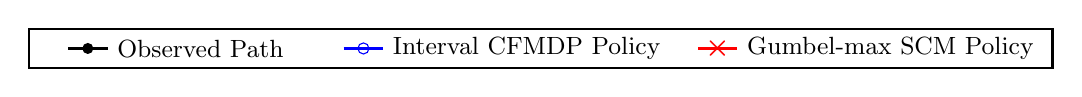
\begin{tikzpicture}[scale=1.0, every node/.style={scale=1.0}]
            \draw[thick, black] (-3, -0.25) rectangle (10, 0.25);
            %
            \draw[black, line width=1pt] (-2.5, 0.0) -- (-2,0.0);
            \fill[black] (-2.25,0.0) circle (2pt); %
            \node[right] at (-2,0.0) {\small Observed Path};
            
            %
            \draw[blue, line width=1pt] (1.0,0.0) -- (1.5,0.0);
            \node[draw=blue, circle, minimum size=4pt, inner sep=0pt] at (1.25,0.0) {}; %
            \node[right] at (1.5,0.0) {\small Interval CFMDP Policy};
            
            %
            \draw[red, line width=1pt] (5.5,0) -- (6,0);
            \node[red] at (5.75,0) {$\boldsymbol{\times}$}; %
            \node[right] at (6,0) {\small Gumbel-max SCM Policy};
        \end{tikzpicture}
    }\\
    %
    \subfigure[\footnotesize Lowest cumulative reward: Interval CFMDP ($312$), Gumbel-max SCM ($312$)]{%
        \resizebox{0.76\columnwidth}{!}{
             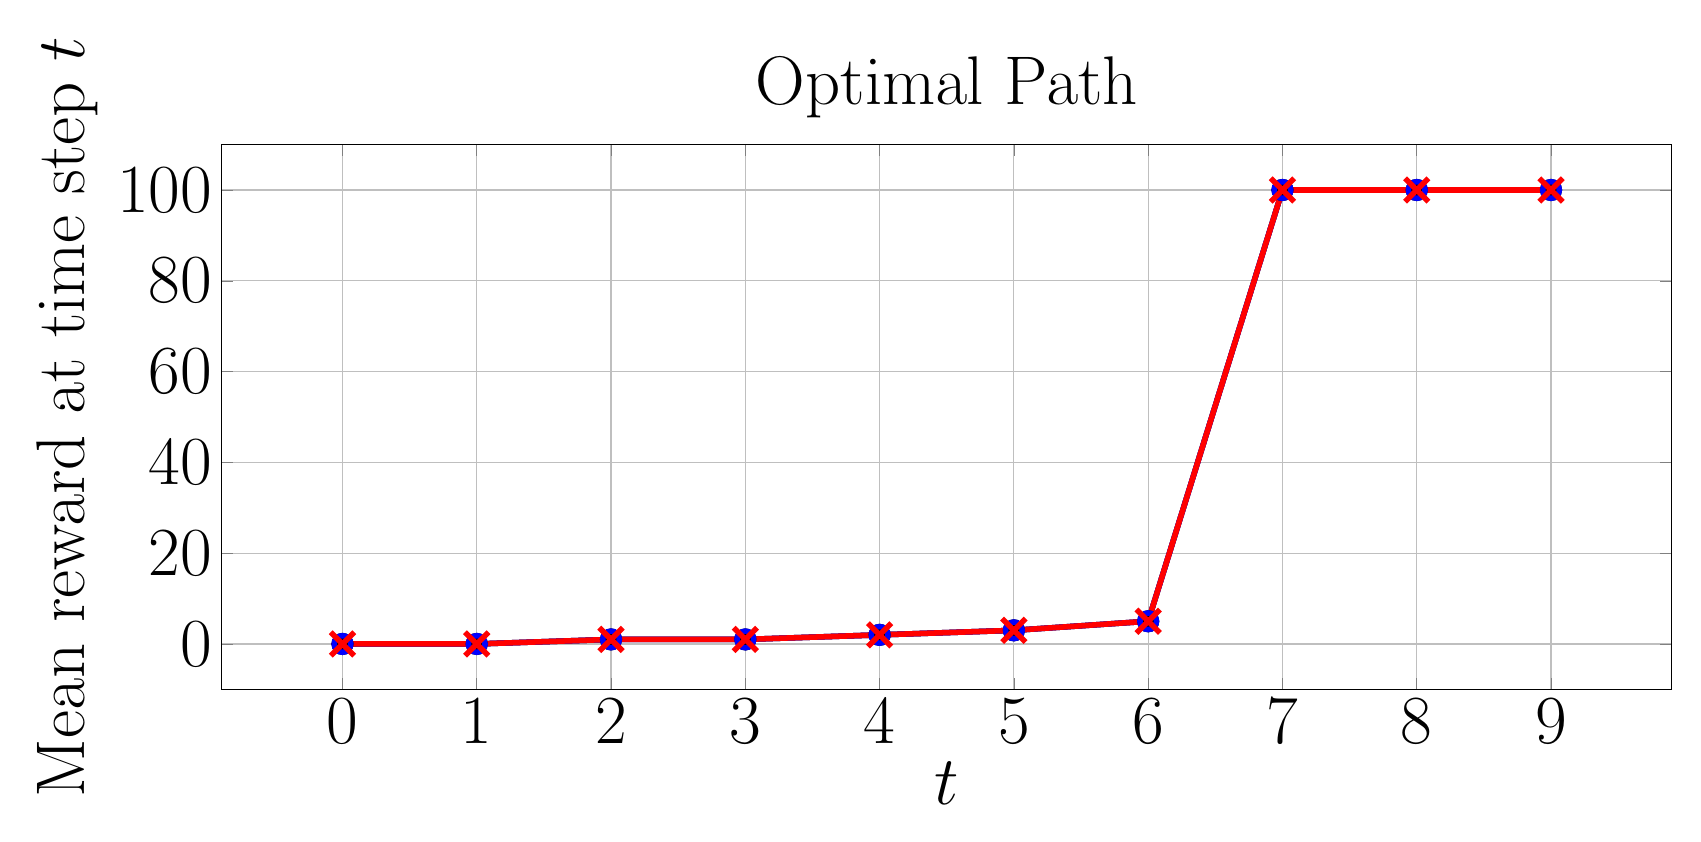
\begin{tikzpicture}
                \begin{axis}[
                    xlabel={$t$},
                    ylabel={Mean reward at time step $t$},
                    title={Optimal Path},
                    grid=both,
                    width=20cm, height=8.5cm,
                    every axis/.style={font=\Huge},
                    %
                ]
                \addplot[
                    color=black, %
                    mark=*, %
                    line width=2pt,
                    mark size=3pt,
                    error bars/.cd,
                    y dir=both, %
                    y explicit, %
                    error bar style={line width=1pt,solid},
                    error mark options={line width=1pt,mark size=4pt,rotate=90}
                ]
                coordinates {
                    (0, 0.0)  +- (0, 0.0)
                    (1, 0.0)  +- (0, 0.0) 
                    (2, 1.0)  +- (0, 0.0) 
                    (3, 1.0)  +- (0, 0.0)
                    (4, 2.0)  +- (0, 0.0)
                    (5, 3.0) +- (0, 0.0)
                    (6, 5.0) +- (0, 0.0)
                    (7, 100.0) +- (0, 0.0)
                    (8, 100.0) +- (0, 0.0)
                    (9, 100.0) +- (0, 0.0)
                };
                %
                \addplot[
                    color=blue, %
                    mark=o, %
                    line width=2pt,
                    mark size=3pt,
                    error bars/.cd,
                    y dir=both, %
                    y explicit, %
                    error bar style={line width=1pt,solid},
                    error mark options={line width=1pt,mark size=4pt,rotate=90}
                ]
                 coordinates {
                    (0, 0.0)  +- (0, 0.0)
                    (1, 0.0)  +- (0, 0.0) 
                    (2, 1.0)  +- (0, 0.0) 
                    (3, 1.0)  +- (0, 0.0)
                    (4, 2.0)  +- (0, 0.0)
                    (5, 3.0) +- (0, 0.0)
                    (6, 5.0) +- (0, 0.0)
                    (7, 100.0) +- (0, 0.0)
                    (8, 100.0) +- (0, 0.0)
                    (9, 100.0) +- (0, 0.0)
                };
                %
                \addplot[
                    color=red, %
                    mark=x, %
                    line width=2pt,
                    mark size=6pt,
                    error bars/.cd,
                    y dir=both, %
                    y explicit, %
                    error bar style={line width=1pt,solid},
                    error mark options={line width=1pt,mark size=4pt,rotate=90}
                ]
                coordinates {
                    (0, 0.0)  +- (0, 0.0)
                    (1, 0.0)  +- (0, 0.0) 
                    (2, 1.0)  +- (0, 0.0) 
                    (3, 1.0)  +- (0, 0.0)
                    (4, 2.0)  +- (0, 0.0)
                    (5, 3.0) +- (0, 0.0)
                    (6, 5.0) +- (0, 0.0)
                    (7, 100.0) +- (0, 0.0)
                    (8, 100.0) +- (0, 0.0)
                    (9, 100.0) +- (0, 0.0)
                };
                \end{axis}
            \end{tikzpicture}
         }
    }
    \hspace{1cm}
    \subfigure[\footnotesize Lowest cumulative reward: Interval CFMDP ($19$), Gumbel-max SCM ($-88$)]{%
         \resizebox{0.76\columnwidth}{!}{
            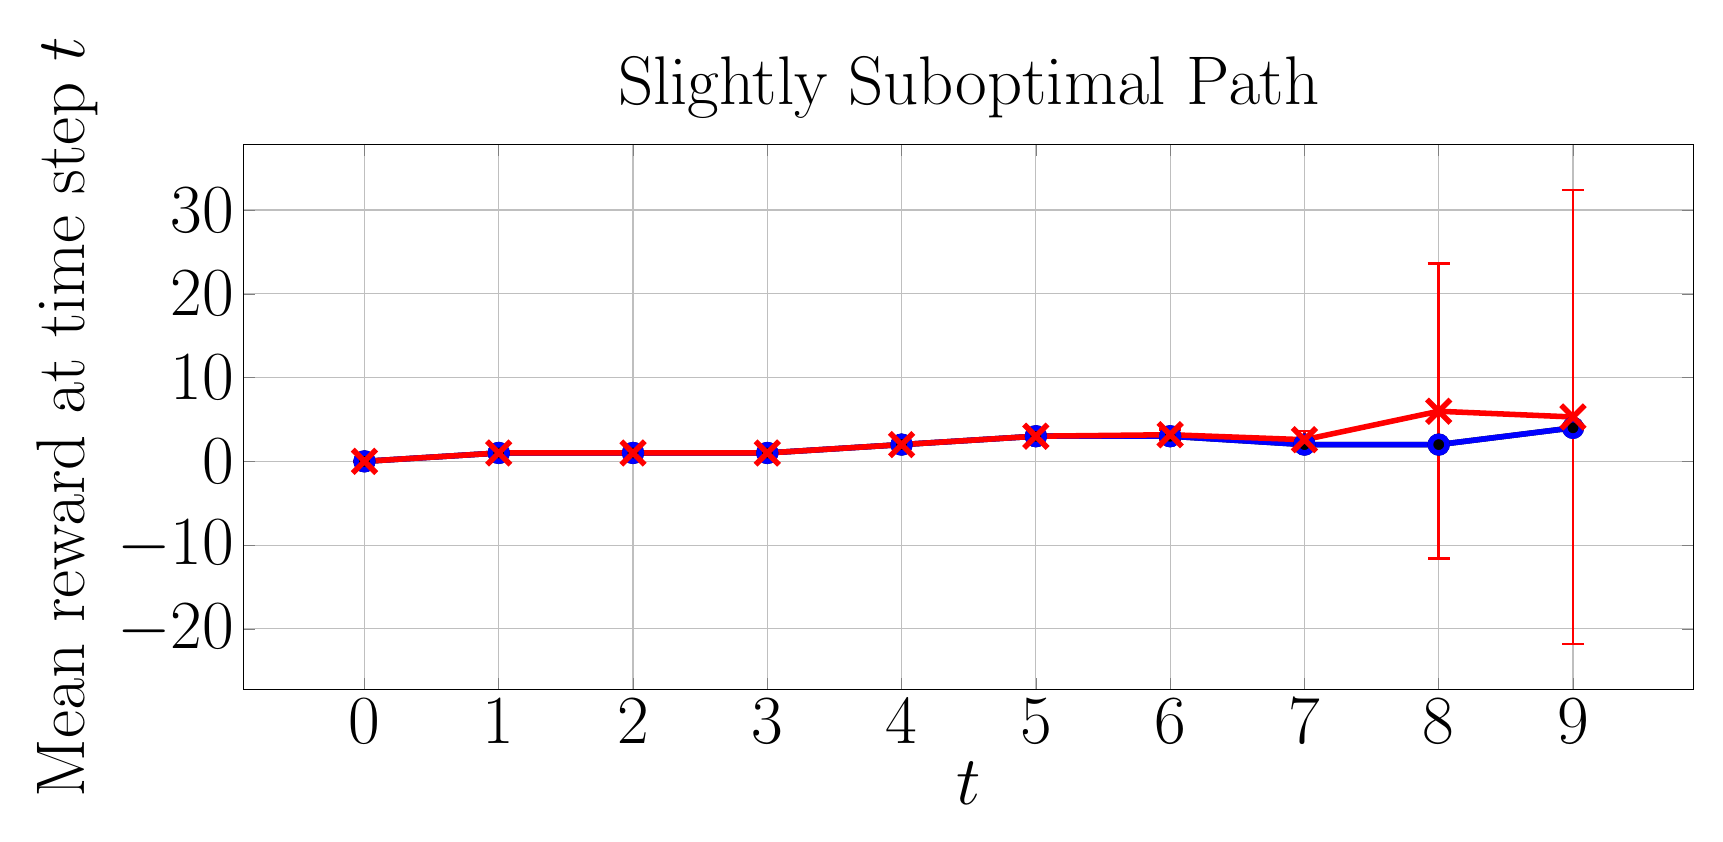
\begin{tikzpicture}
                \begin{axis}[
                    xlabel={$t$},
                    ylabel={Mean reward at time step $t$},
                    title={Slightly Suboptimal Path},
                    grid=both,
                    width=20cm, height=8.5cm,
                    every axis/.style={font=\Huge},
                    %
                ]
                \addplot[
                    color=black, %
                    mark=*, %
                    line width=2pt,
                    mark size=3pt,
                    error bars/.cd,
                    y dir=both, %
                    y explicit, %
                    error bar style={line width=1pt,solid},
                    error mark options={line width=1pt,mark size=4pt,rotate=90}
                ]
              coordinates {
                    (0, 0.0)  +- (0, 0.0)
                    (1, 1.0)  +- (0, 0.0) 
                    (2, 1.0)  +- (0, 0.0) 
                    (3, 1.0)  +- (0, 0.0)
                    (4, 2.0)  +- (0, 0.0)
                    (5, 3.0) +- (0, 0.0)
                    (6, 3.0) +- (0, 0.0)
                    (7, 2.0) +- (0, 0.0)
                    (8, 2.0) +- (0, 0.0)
                    (9, 4.0) +- (0, 0.0)
                };
                %
                \addplot[
                    color=blue, %
                    mark=o, %
                    line width=2pt,
                    mark size=3pt,
                    error bars/.cd,
                    y dir=both, %
                    y explicit, %
                    error bar style={line width=1pt,solid},
                    error mark options={line width=1pt,mark size=4pt,rotate=90}
                ]
              coordinates {
                    (0, 0.0)  +- (0, 0.0)
                    (1, 1.0)  +- (0, 0.0) 
                    (2, 1.0)  +- (0, 0.0) 
                    (3, 1.0)  +- (0, 0.0)
                    (4, 2.0)  +- (0, 0.0)
                    (5, 3.0) +- (0, 0.0)
                    (6, 3.0) +- (0, 0.0)
                    (7, 2.0) +- (0, 0.0)
                    (8, 2.0) +- (0, 0.0)
                    (9, 4.0) +- (0, 0.0)
                };
                %
                \addplot[
                    color=red, %
                    mark=x, %
                    line width=2pt,
                    mark size=6pt,
                    error bars/.cd,
                    y dir=both, %
                    y explicit, %
                    error bar style={line width=1pt,solid},
                    error mark options={line width=1pt,mark size=4pt,rotate=90}
                ]
                coordinates {
                    (0, 0.0)  +- (0, 0.0)
                    (1, 1.0)  +- (0, 0.0) 
                    (2, 1.0)  +- (0, 0.0) 
                    (3, 1.0)  +- (0, 0.0)
                    (4, 2.0)  += (0, 0.0)
                    (5, 3.0)  += (0, 0.0)
                    (6, 3.17847) += (0, 0.62606746) -= (0, 0.62606746)
                    (7, 2.5832885) += (0, 1.04598233) -= (0, 1.04598233)
                    (8, 5.978909) += (0, 17.60137623) -= (0, 17.60137623)
                    (9, 5.297059) += (0, 27.09227512) -= (0, 27.09227512)
                };
                \end{axis}
            \end{tikzpicture}
         }
    }\\[-1.5pt]
    \subfigure[\footnotesize Lowest cumulative reward: Interval CFMDP ($14$), Gumbel-max SCM ($-598$)]{%
         \resizebox{0.76\columnwidth}{!}{
             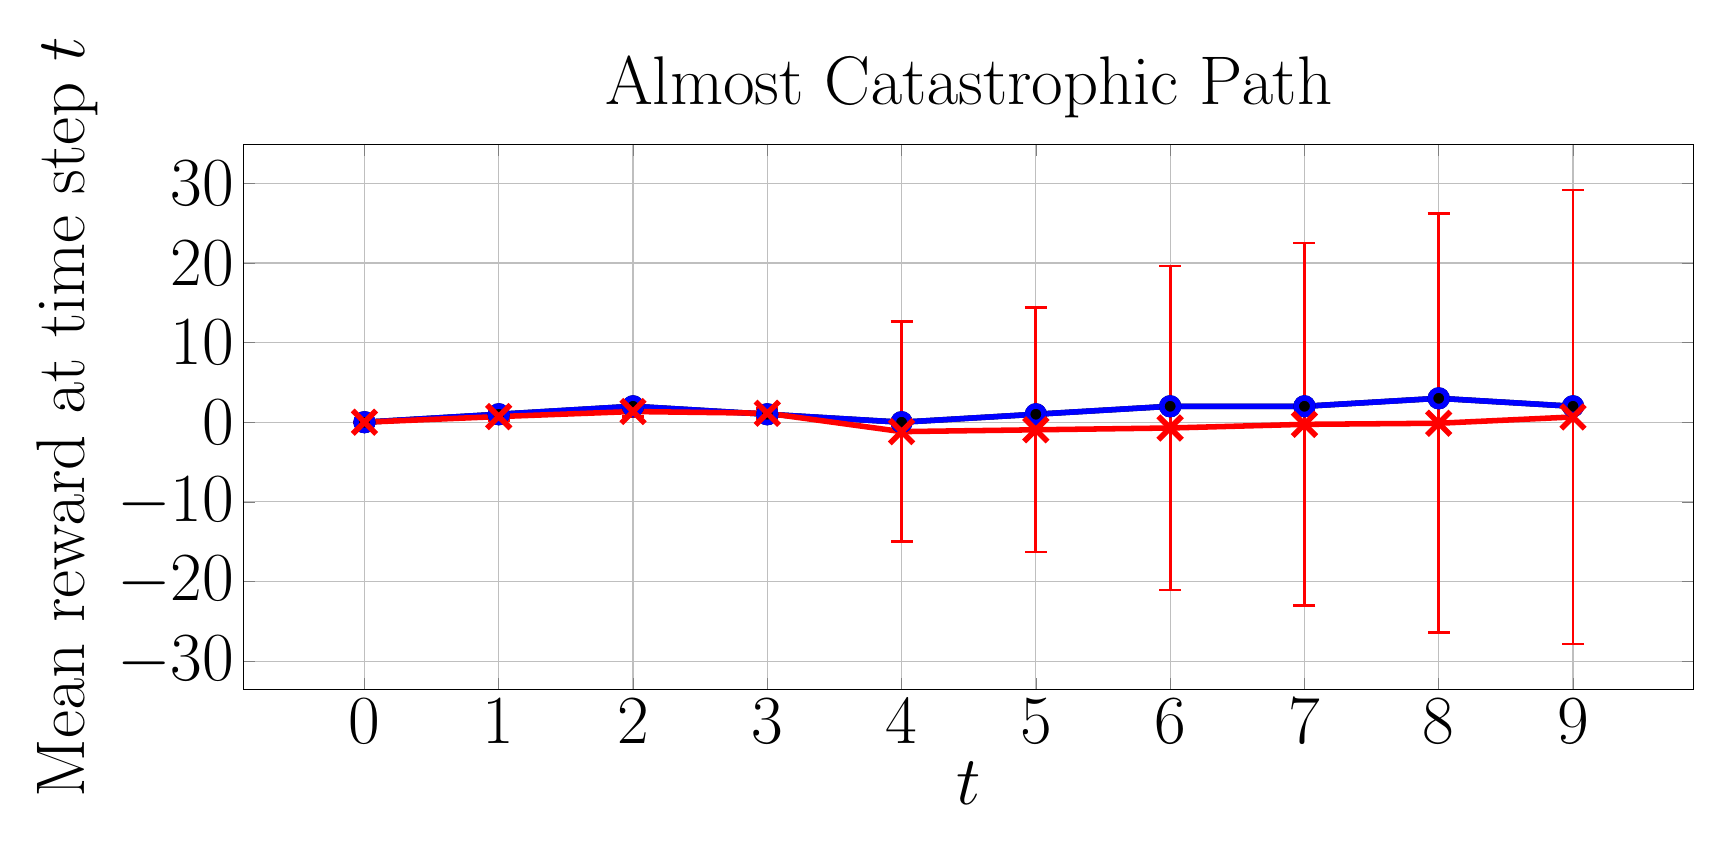
\begin{tikzpicture}
                \begin{axis}[
                    xlabel={$t$},
                    ylabel={Mean reward at time step $t$},
                    title={Almost Catastrophic Path},
                    grid=both,
                    width=20cm, height=8.5cm,
                    every axis/.style={font=\Huge},
                    %
                ]
                \addplot[
                    color=black, %
                    mark=*, %
                    line width=2pt,
                    mark size=3pt,
                    error bars/.cd,
                    y dir=both, %
                    y explicit, %
                    error bar style={line width=1pt,solid},
                    error mark options={line width=1pt,mark size=4pt,rotate=90}
                ]
                coordinates {
                    (0, 0.0)  +- (0, 0.0)
                    (1, 1.0)  +- (0, 0.0) 
                    (2, 2.0)  +- (0, 0.0) 
                    (3, 1.0)  +- (0, 0.0)
                    (4, 0.0)  +- (0, 0.0)
                    (5, 1.0) +- (0, 0.0)
                    (6, 2.0) +- (0, 0.0)
                    (7, 2.0) +- (0, 0.0)
                    (8, 3.0) +- (0, 0.0)
                    (9, 2.0) +- (0, 0.0)
                };
                %
                \addplot[
                    color=blue, %
                    mark=o, %
                    line width=2pt,
                    mark size=3pt,
                    error bars/.cd,
                    y dir=both, %
                    y explicit, %
                    error bar style={line width=1pt,solid},
                    error mark options={line width=1pt,mark size=4pt,rotate=90}
                ]
                coordinates {
                    (0, 0.0)  +- (0, 0.0)
                    (1, 1.0)  +- (0, 0.0) 
                    (2, 2.0)  +- (0, 0.0) 
                    (3, 1.0)  +- (0, 0.0)
                    (4, 0.0)  +- (0, 0.0)
                    (5, 1.0) +- (0, 0.0)
                    (6, 2.0) +- (0, 0.0)
                    (7, 2.0) +- (0, 0.0)
                    (8, 3.0) +- (0, 0.0)
                    (9, 2.0) +- (0, 0.0)
                };
                %
                \addplot[
                    color=red, %
                    mark=x, %
                    line width=2pt,
                    mark size=6pt,
                    error bars/.cd,
                    y dir=both, %
                    y explicit, %
                    error bar style={line width=1pt,solid},
                    error mark options={line width=1pt,mark size=4pt,rotate=90}
                ]
                coordinates {
                    (0, 0.0)  +- (0, 0.0)
                    (1, 0.7065655)  +- (0, 0.4553358) 
                    (2, 1.341673)  +- (0, 0.67091621) 
                    (3, 1.122926)  +- (0, 0.61281824)
                    (4, -1.1821935)  +- (0, 13.82444042)
                    (5, -0.952399)  +- (0, 15.35195457)
                    (6, -0.72672) +- (0, 20.33508414)
                    (7, -0.268983) +- (0, 22.77861454)
                    (8, -0.1310835) +- (0, 26.31013314)
                    (9, 0.65806) +- (0, 28.50670214)
                };
                %
            %
            %
            %
            %
            %
            %
            %
            %
            %
            %
            %
            %
            %
            %
            %
            %
            %
            %
                \end{axis}
            \end{tikzpicture}
         }
    }
    \hspace{1cm}
    \subfigure[\footnotesize Lowest cumulative reward: Interval CFMDP ($-698$), Gumbel-max SCM ($-698$)]{%
         \resizebox{0.76\columnwidth}{!}{
            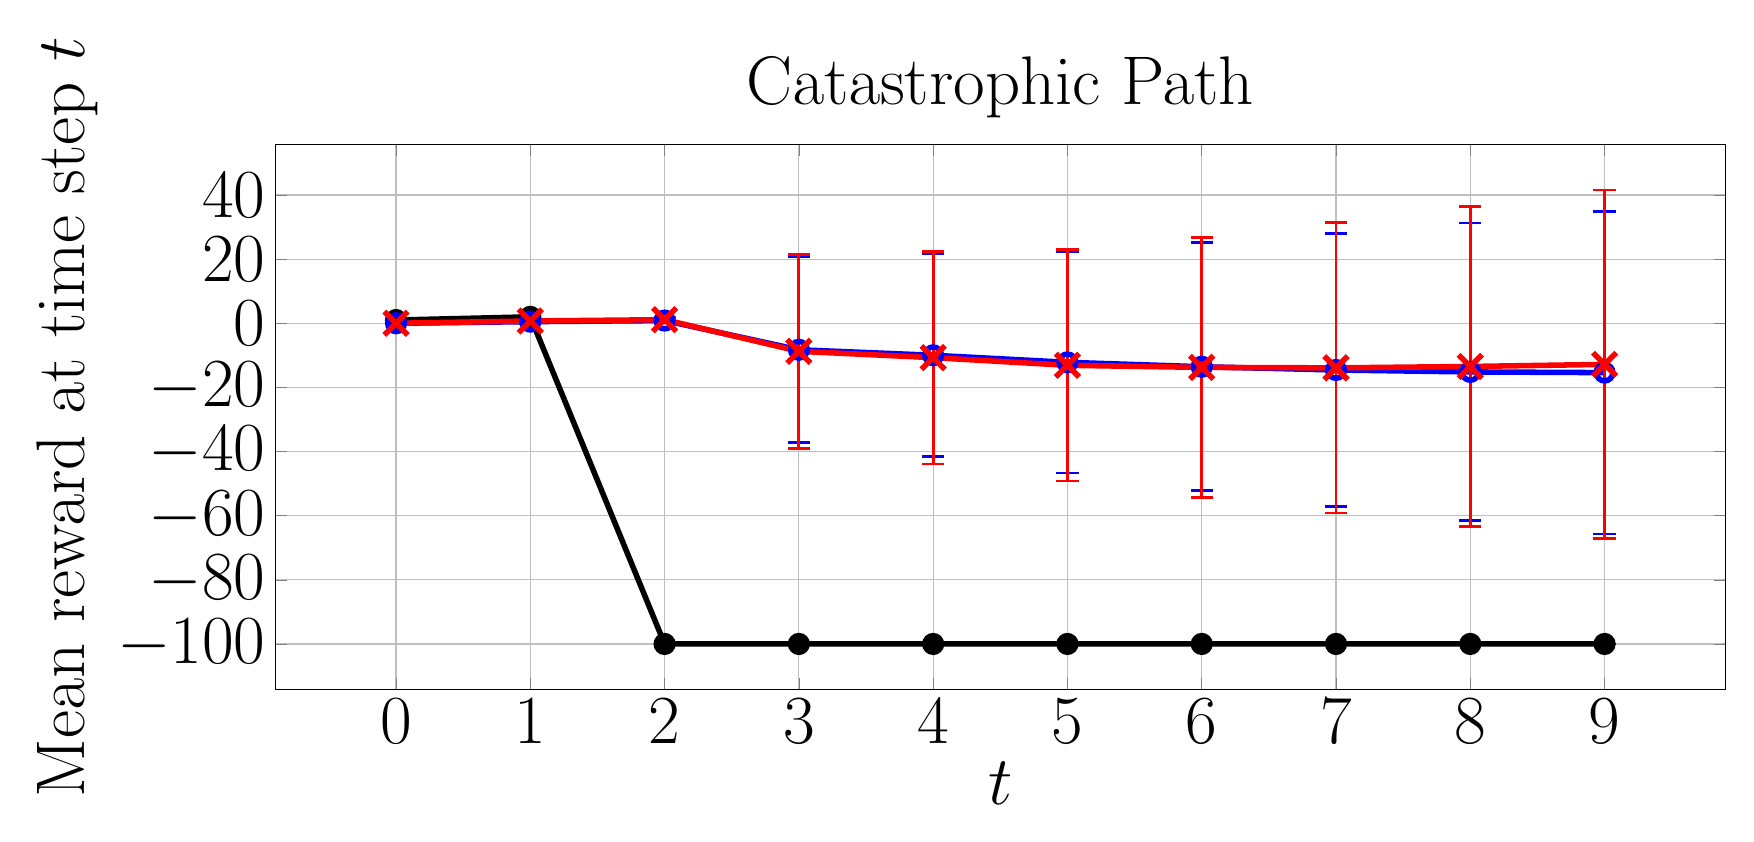
\begin{tikzpicture}
                \begin{axis}[
                    xlabel={$t$},
                    ylabel={Mean reward at time step $t$},
                    title={Catastrophic Path},
                    grid=both,
                    width=20cm, height=8.5cm,
                    every axis/.style={font=\Huge},
                    %
                ]
                \addplot[
                    color=black, %
                    mark=*, %
                    line width=2pt,
                    mark size=3pt,
                    error bars/.cd,
                    y dir=both, %
                    y explicit, %
                    error bar style={line width=1pt,solid},
                    error mark options={line width=1pt,mark size=4pt,rotate=90}
                ]
                coordinates {
                    (0, 1.0)  +- (0, 0.0)
                    (1, 2.0)  +- (0, 0.0) 
                    (2, -100.0)  +- (0, 0.0) 
                    (3, -100.0)  +- (0, 0.0)
                    (4, -100.0)  +- (0, 0.0)
                    (5, -100.0) +- (0, 0.0)
                    (6, -100.0) +- (0, 0.0)
                    (7, -100.0) +- (0, 0.0)
                    (8, -100.0) +- (0, 0.0)
                    (9, -100.0) +- (0, 0.0)
                };
                %
                \addplot[
                    color=blue, %
                    mark=o, %
                    line width=2pt,
                    mark size=3pt,
                    error bars/.cd,
                    y dir=both, %
                    y explicit, %
                    error bar style={line width=1pt,solid},
                    error mark options={line width=1pt,mark size=4pt,rotate=90}
                ]
                coordinates {
                    (0, 0.0)  +- (0, 0.0)
                    (1, 0.504814)  +- (0, 0.49997682) 
                    (2, 0.8439835)  +- (0, 0.76831917) 
                    (3, -8.2709165)  +- (0, 28.93656754)
                    (4, -9.981082)  +- (0, 31.66825363)
                    (5, -12.1776325) +- (0, 34.53463233)
                    (6, -13.556076) +- (0, 38.62845372)
                    (7, -14.574418) +- (0, 42.49603359)
                    (8, -15.1757075) +- (0, 46.41913968)
                    (9, -15.3900395) +- (0, 50.33563368)
                };
                %
                \addplot[
                    color=red, %
                    mark=x, %
                    line width=2pt,
                    mark size=6pt,
                    error bars/.cd,
                    y dir=both, %
                    y explicit, %
                    error bar style={line width=1pt,solid},
                    error mark options={line width=1pt,mark size=4pt,rotate=90}
                ]
                coordinates {
                    (0, 0.0)  +- (0, 0.0)
                    (1, 0.701873)  +- (0, 0.45743556) 
                    (2, 1.1227805)  +- (0, 0.73433129) 
                    (3, -8.7503255)  +- (0, 30.30257976)
                    (4, -10.722092)  +- (0, 33.17618589)
                    (5, -13.10721)  +- (0, 36.0648089)
                    (6, -13.7631645) +- (0, 40.56553451)
                    (7, -13.909043) +- (0, 45.23829402)
                    (8, -13.472517) +- (0, 49.96270296)
                    (9, -12.8278835) +- (0, 54.38618735)
                };
                %
            %
            %
            %
            %
            %
            %
            %
            %
            %
            %
            %
            %
            %
            %
            %
            %
            %
            %
                \end{axis}
            \end{tikzpicture}
         }
    }
    \caption{Average instant reward of CF paths induced by policies on GridWorld $p=0.4$.}
    \label{fig: reward p=0.4}
\end{figure*}

\subsection{Experimental Setup}
To compare policy performance, we measure the average rewards of counterfactual paths induced by our policy and the Gumbel-max policy by uniformly sampling $200$ counterfactual MDPs from the ICFMDP and generating $10,000$ counterfactual paths over each sampled CFMDP. \jl{Since the interval CFMDP depends on the observed path, we select $4$  paths of varying optimality to evaluate how the observed path impacts the performance of both policies: an optimal path, a slightly suboptimal path that could reach the optimal reward with a few changes, a catastrophic path that enters a catastrophic, terminal state with low reward, and an almost catastrophic path that was close to entering a catastrophic state.} When measuring the average probability bound widths and execution time needed to generate the ICFMDPs, we averaged over $20$ randomly generated observed paths
\footnote{Further training details are provided in Appendix \ref{app: training details}, and the code is provided at \href{https://github.com/ddv-lab/robust-cf-inference-in-MDPs}{https://github.com/ddv-lab/robust-cf-inference-in-MDPs}
%
%
.}.

\subsection{GridWorld}
\jl{The GridWorld MDP is a $4 \times 4$ grid where an agent must navigate from the top-left corner to the goal state in the bottom-right corner, avoiding a dangerous terminal state in the centre. At each time step, the agent can move up, down, left, or right, but there is a small probability (controlled by hyper-parameter $p$) of moving in an unintended direction. As the agent nears the goal, the reward for each state increases, culminating in a reward of $+100$ for reaching the goal. Entering the dangerous state results in a penalty of $-100$. We use two versions of GridWorld: a less stochastic version with $p=0.9$ (i.e., $90$\% chance of moving in the chosen direction) and a more stochastic version with $p=0.4$.}

\paragraph{GridWorld ($p=0.9$)}
When $p=0.9$, the counterfactual probability bounds are typically narrow (see Table \ref{tab:nonzero_probs} for average measurements). Consequently, as shown in Figure \ref{fig: reward p=0.9}, both policies are nearly identical and perform similarly well across the optimal, slightly suboptimal, and catastrophic paths.
%
However, for the almost catastrophic path, the interval CFMDP path is more conservative and follows the observed path more closely (as this is where the probability bounds are narrowest), which typically requires one additional step to reach the goal state than the Gumbel-max SCM policy.
%

\paragraph{GridWorld ($p=0.4$)}
\jl{When $p=0.4$, the GridWorld environment becomes more uncertain, increasing the risk of entering the dangerous state even if correct actions are chosen. Thus, as shown in Figure \ref{fig: reward p=0.4}, the interval CFMDP policy adopts a more conservative approach, avoiding deviation from the observed policy if it cannot guarantee higher counterfactual rewards (see the slightly suboptimal and almost catastrophic paths), whereas the Gumbel-max SCM is inconsistent: it can yield higher rewards, but also much lower rewards, reflected in the wide error bars.} For the catastrophic path, both policies must deviate from the observed path to achieve a higher reward and, in this case, perform similarly.
%
%
%
%
\subsection{Sepsis}
The Sepsis MDP \citep{oberst2019counterfactual} simulates trajectories of Sepsis patients. Each state consists of four vital signs (heart rate, blood pressure, oxygen concentration, and glucose levels), categorised as low, normal, or high.
and three treatments that can be toggled on/off at each time step (8 actions in total). Unlike \citet{oberst2019counterfactual}, we scale rewards based on the number of out-of-range vital signs, between $-1000$ (patient dies) and $1000$ (patient discharged). \jl{Like the GridWorld $p=0.4$ experiment, the Sepsis MDP is highly uncertain, as many states are equally likely to lead to optimal and poor outcomes. Thus, as shown in Figure \ref{fig: reward sepsis}, both policies follow the observed optimal and almost catastrophic paths to guarantee rewards are no worse than the observation.} However, improving the catastrophic path requires deviating from the observation. Here, the Gumbel-max SCM policy, on average, performs better than the interval CFMDP policy. But, since both policies have lower bounds clipped at $-1000$, neither policy reliably improves over the observation. In contrast, for the slightly suboptimal path, the interval CFMDP policy performs significantly better, shown by its higher lower bounds. 
Moreover, in these two cases, the worst-case counterfactual path generated by the interval CFMDP policy is better than that of the Gumbel-max SCM policy,
indicating its greater robustness.
%
\begin{figure*}
    \centering
     \resizebox{0.6\textwidth}{!}{
        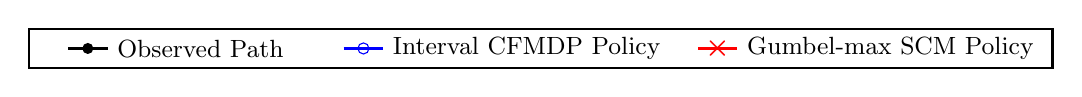
\begin{tikzpicture}[scale=1.0, every node/.style={scale=1.0}]
            \draw[thick, black] (-3, -0.25) rectangle (10, 0.25);
            %
            \draw[black, line width=1pt] (-2.5, 0.0) -- (-2,0.0);
            \fill[black] (-2.25,0.0) circle (2pt); %
            \node[right] at (-2,0.0) {\small Observed Path};
            
            %
            \draw[blue, line width=1pt] (1.0,0.0) -- (1.5,0.0);
            \node[draw=blue, circle, minimum size=4pt, inner sep=0pt] at (1.25,0.0) {}; %
            \node[right] at (1.5,0.0) {\small Interval CFMDP Policy};
            
            %
            \draw[red, line width=1pt] (5.5,0) -- (6,0);
            \node[red] at (5.75,0) {$\boldsymbol{\times}$}; %
            \node[right] at (6,0) {\small Gumbel-max SCM Policy};
        \end{tikzpicture}
    }\\
    \subfigure[\footnotesize Lowest cumulative reward: Interval CFMDP ($8000$), Gumbel-max SCM ($8000$)]{%
         \resizebox{0.76\columnwidth}{!}{
             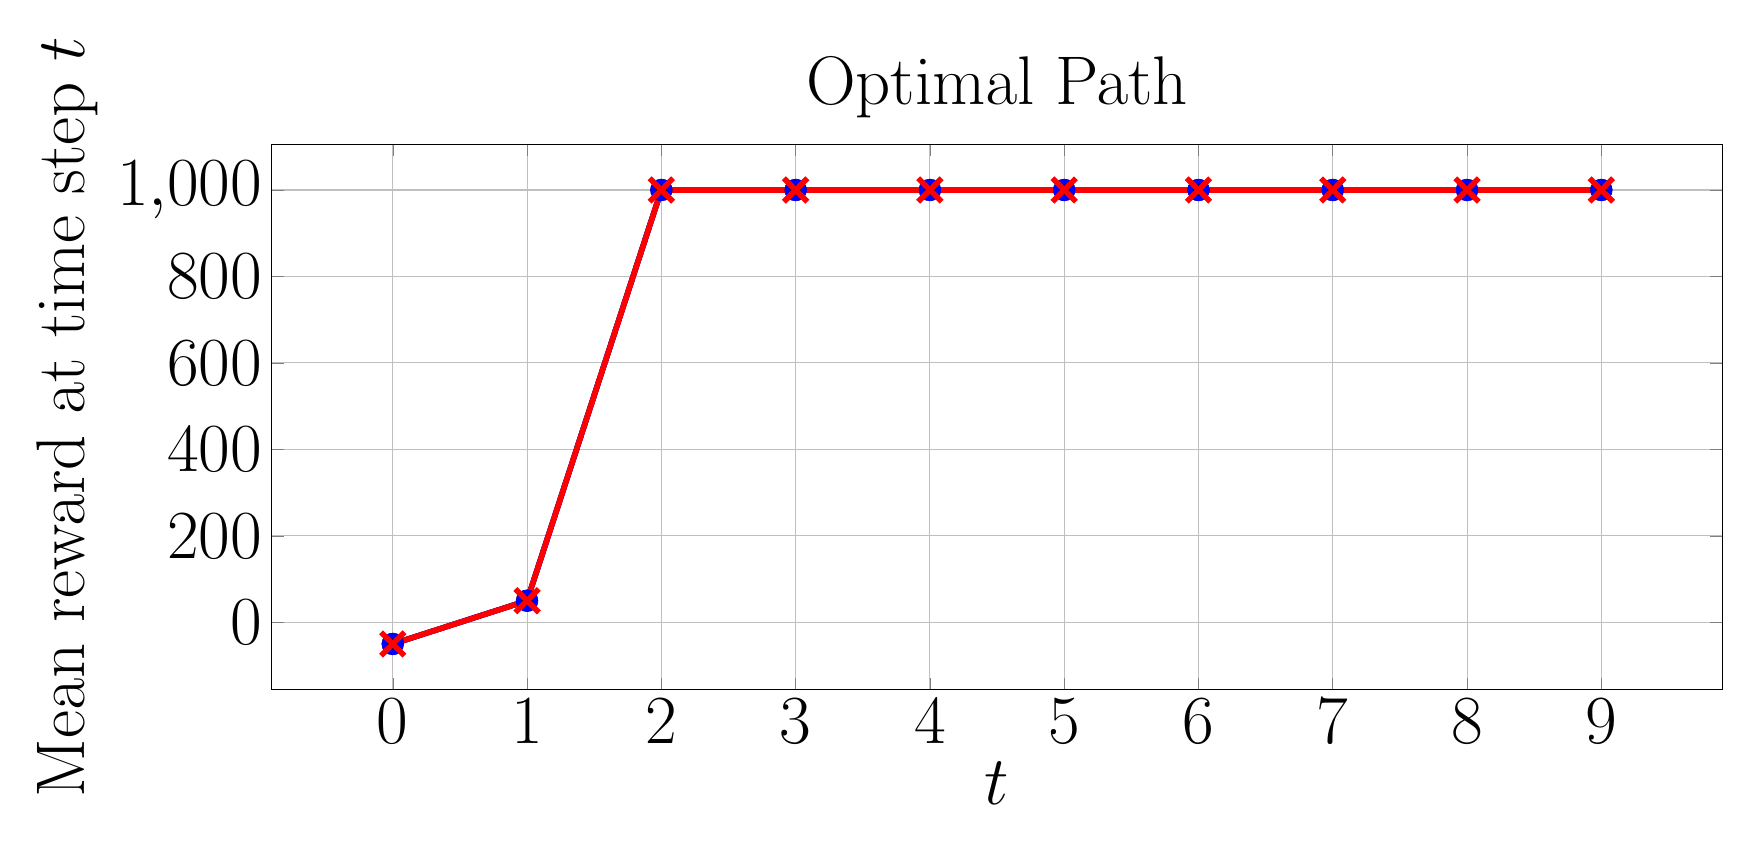
\begin{tikzpicture}
                \begin{axis}[
                    xlabel={$t$},
                    ylabel={Mean reward at time step $t$},
                    title={Optimal Path},
                    grid=both,
                    width=20cm, height=8.5cm,
                    every axis/.style={font=\Huge},
                    %
                ]
                \addplot[
                    color=black, %
                    mark=*, %
                    line width=2pt,
                    mark size=3pt,
                ]
                coordinates {
                    (0, -50.0)
                    (1, 50.0)
                    (2, 1000.0)
                    (3, 1000.0)
                    (4, 1000.0)
                    (5, 1000.0)
                    (6, 1000.0)
                    (7, 1000.0)
                    (8, 1000.0)
                    (9, 1000.0)
                };
                %
                \addplot[
                    color=blue, %
                    mark=o, %
                    line width=2pt,
                    mark size=3pt,
                    error bars/.cd,
                    y dir=both, %
                    y explicit, %
                    error bar style={line width=1pt,solid},
                    error mark options={line width=1pt,mark size=4pt,rotate=90}
                ]
                coordinates {
                    (0, -50.0)  +- (0, 0.0)
                    (1, 50.0)  +- (0, 0.0) 
                    (2, 1000.0)  +- (0, 0.0) 
                    (3, 1000.0)  +- (0, 0.0)
                    (4, 1000.0)  +- (0, 0.0)
                    (5, 1000.0) +- (0, 0.0)
                    (6, 1000.0) +- (0, 0.0)
                    (7, 1000.0) +- (0, 0.0)
                    (8, 1000.0) +- (0, 0.0)
                    (9, 1000.0) +- (0, 0.0)
                };
                %
                \addplot[
                    color=red, %
                    mark=x, %
                    line width=2pt,
                    mark size=6pt,
                    error bars/.cd,
                    y dir=both, %
                    y explicit, %
                    error bar style={line width=1pt,solid},
                    error mark options={line width=1pt,mark size=4pt,rotate=90}
                ]
                coordinates {
                    (0, -50.0)  +- (0, 0.0)
                    (1, 50.0)  +- (0, 0.0) 
                    (2, 1000.0)  +- (0, 0.0) 
                    (3, 1000.0)  +- (0, 0.0)
                    (4, 1000.0)  +- (0, 0.0)
                    (5, 1000.0) +- (0, 0.0)
                    (6, 1000.0) +- (0, 0.0)
                    (7, 1000.0) +- (0, 0.0)
                    (8, 1000.0) +- (0, 0.0)
                    (9, 1000.0) +- (0, 0.0)
                };
                %
                \end{axis}
            \end{tikzpicture}
         }
    }
    \hspace{1cm}
    \subfigure[\footnotesize Lowest cumulative reward: Interval CFMDP ($-5980$), Gumbel-max SCM ($-8000$)]{%
         \resizebox{0.76\columnwidth}{!}{
            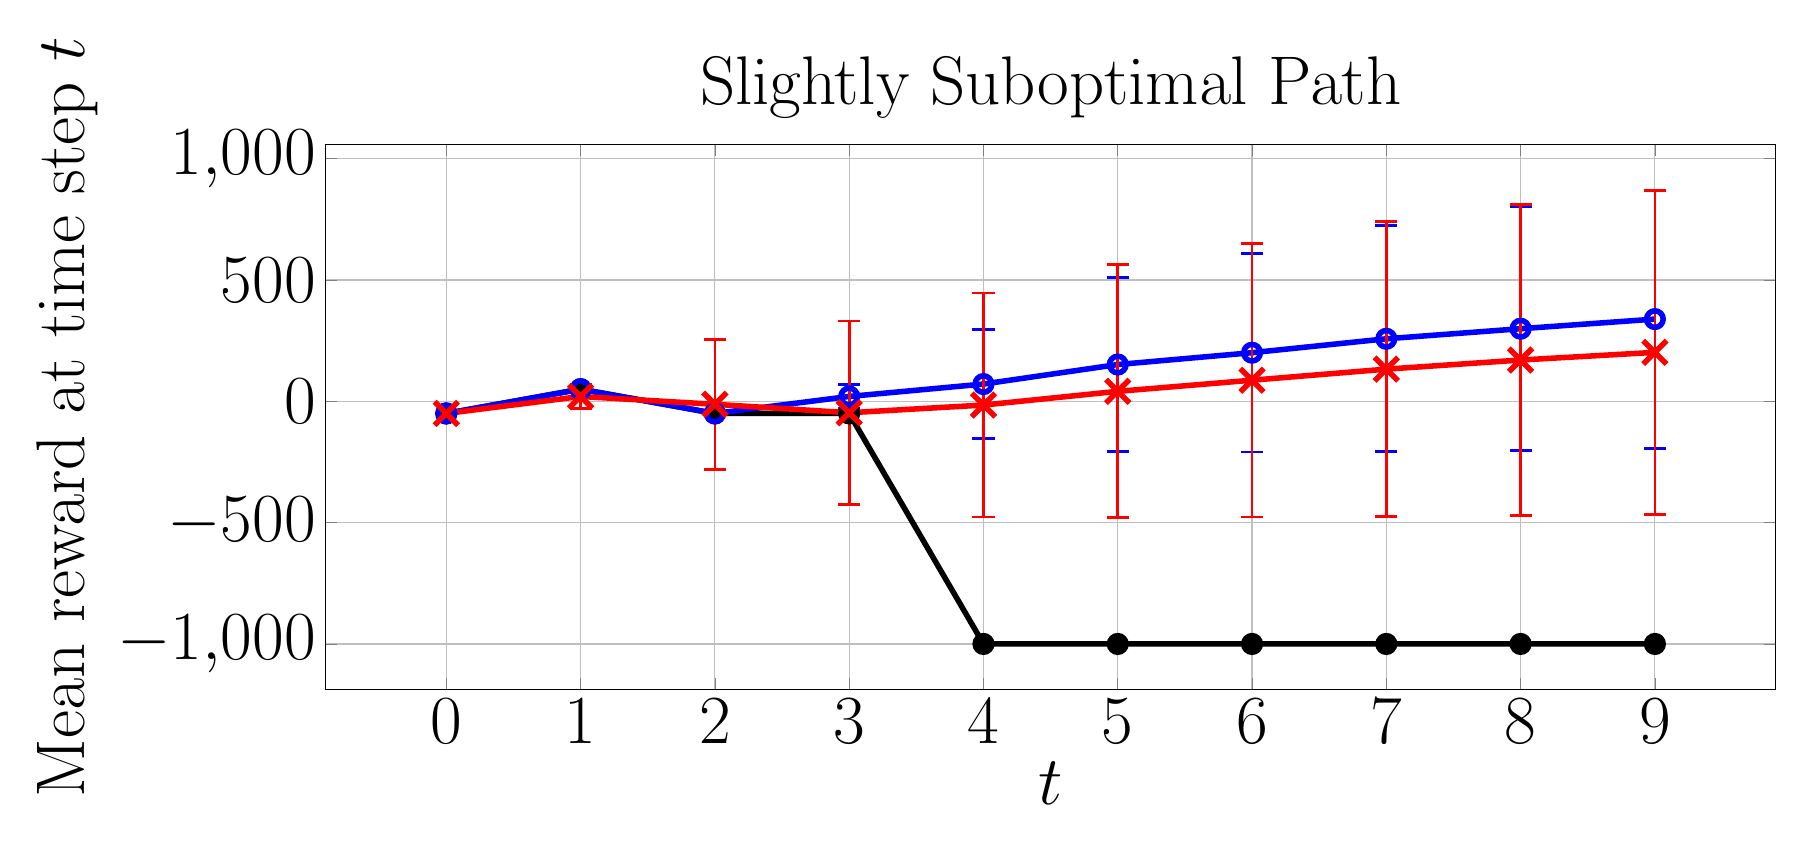
\begin{tikzpicture}
                \begin{axis}[
                    xlabel={$t$},
                    ylabel={Mean reward at time step $t$},
                    title={Slightly Suboptimal Path},
                    grid=both,
                    width=20cm, height=8.5cm,
                    every axis/.style={font=\Huge},
                    %
                ]
               \addplot[
                    color=black, %
                    mark=*, %
                    line width=2pt,
                    mark size=3pt,
                ]
                coordinates {
                    (0, -50.0)
                    (1, 50.0)
                    (2, -50.0)
                    (3, -50.0)
                    (4, -1000.0)
                    (5, -1000.0)
                    (6, -1000.0)
                    (7, -1000.0)
                    (8, -1000.0)
                    (9, -1000.0)
                };
                %
                \addplot[
                    color=blue, %
                    mark=o, %
                    line width=2pt,
                    mark size=3pt,
                    error bars/.cd,
                    y dir=both, %
                    y explicit, %
                    error bar style={line width=1pt,solid},
                    error mark options={line width=1pt,mark size=4pt,rotate=90}
                ]
                coordinates {
                    (0, -50.0)  +- (0, 0.0)
                    (1, 50.0)  +- (0, 0.0) 
                    (2, -50.0)  +- (0, 0.0) 
                    (3, 20.0631)  +- (0, 49.97539413)
                    (4, 71.206585)  +- (0, 226.02033693)
                    (5, 151.60797) +- (0, 359.23292559)
                    (6, 200.40593) +- (0, 408.86185176)
                    (7, 257.77948) +- (0, 466.10372804)
                    (8, 299.237465) +- (0, 501.82579506)
                    (9, 338.9129) +- (0, 532.06124996)
                };
                %
                \addplot[
                    color=red, %
                    mark=x, %
                    line width=2pt,
                    mark size=6pt,
                    error bars/.cd,
                    y dir=both, %
                    y explicit, %
                    error bar style={line width=1pt,solid},
                    error mark options={line width=1pt,mark size=4pt,rotate=90}
                ]
                coordinates {
                    (0, -50.0)  +- (0, 0.0)
                    (1, 20.00736)  +- (0, 49.99786741) 
                    (2, -12.282865)  +- (0, 267.598755) 
                    (3, -47.125995)  +- (0, 378.41755832)
                    (4, -15.381965)  +- (0, 461.77616558)
                    (5, 41.15459) +- (0, 521.53189262)
                    (6, 87.01595) +- (0, 564.22243126 )
                    (7, 132.62376) +- (0, 607.31338037)
                    (8, 170.168145) +- (0, 641.48013693)
                    (9, 201.813135) +- (0, 667.29441777)
                };
                %
                %
                %
                %
                %
                %
                %
                %
                %
                %
                %
                %
                %
                %
                %
                %
                %
                %
                %
                \end{axis}
            \end{tikzpicture}
         }
    }\\[-1.5pt]
    \subfigure[\footnotesize Lowest cumulative reward: Interval CFMDP ($100$), Gumbel-max SCM ($100$)]{%
         \resizebox{0.76\columnwidth}{!}{
             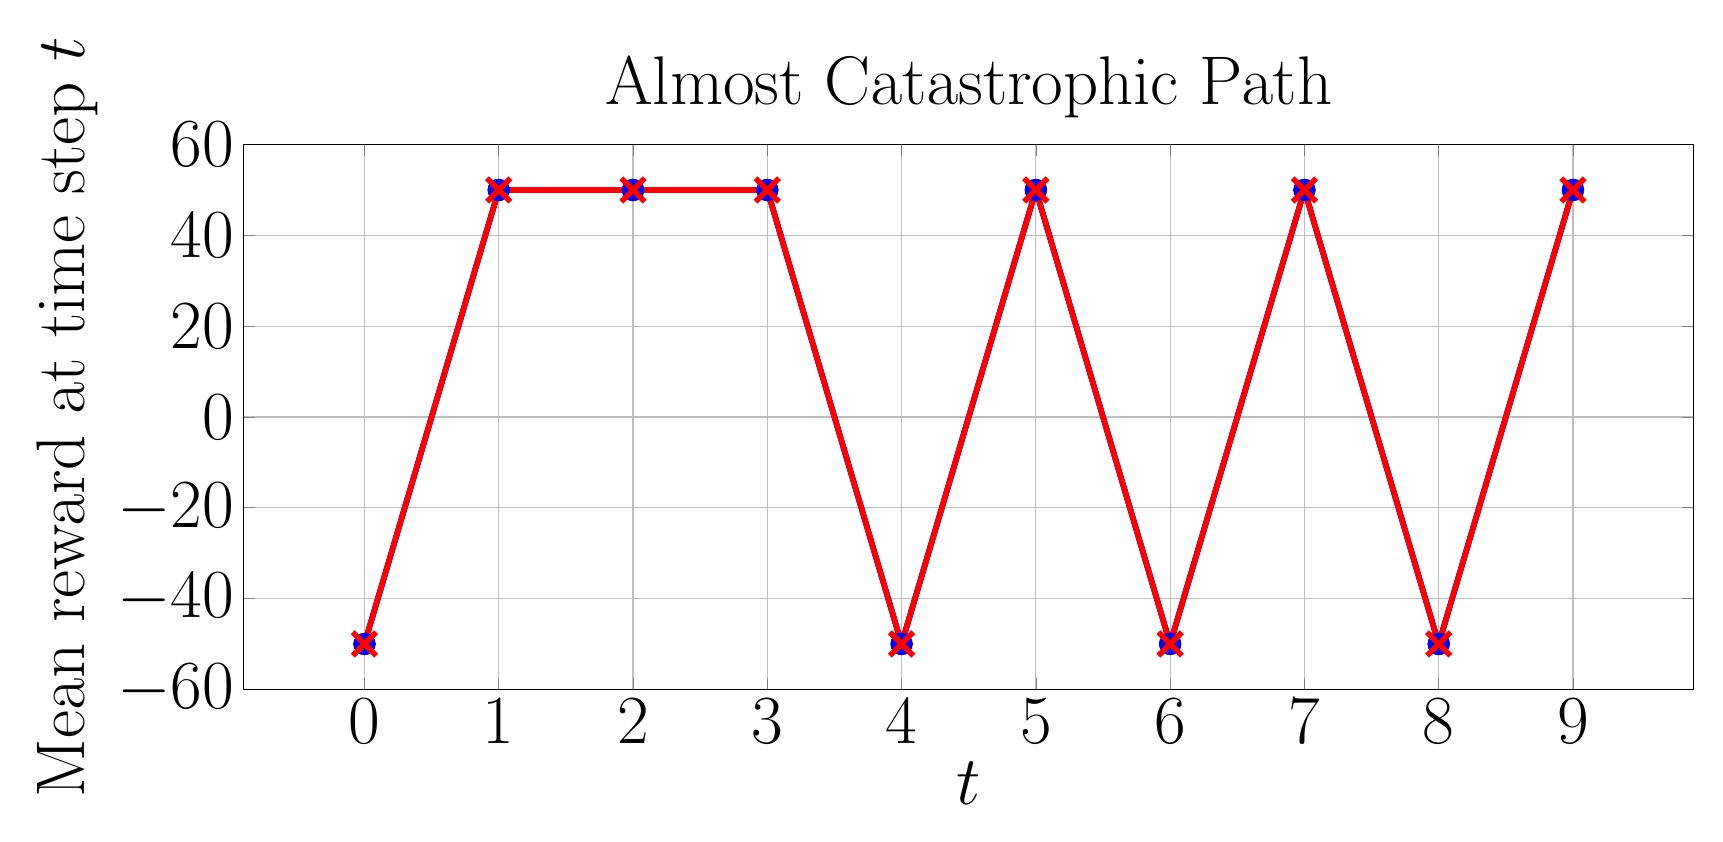
\begin{tikzpicture}
                \begin{axis}[
                    xlabel={$t$},
                    ylabel={Mean reward at time step $t$},
                    title={Almost Catastrophic Path},
                    grid=both,
                    every axis/.style={font=\Huge},
                    width=20cm, height=8.5cm,
                    %
                ]
               \addplot[
                    color=black, %
                    mark=*, %
                    line width=2pt,
                    mark size=3pt,
                ]
                coordinates {
                    (0, -50.0)
                    (1, 50.0)
                    (2, 50.0)
                    (3, 50.0)
                    (4, -50.0)
                    (5, 50.0)
                    (6, -50.0)
                    (7, 50.0)
                    (8, -50.0)
                    (9, 50.0)
                };
                %
                %
                \addplot[
                    color=blue, %
                    mark=o, %
                    line width=2pt,
                    mark size=3pt,
                    error bars/.cd,
                    y dir=both, %
                    y explicit, %
                    error bar style={line width=1pt,solid},
                    error mark options={line width=1pt,mark size=4pt,rotate=90}
                ]
                coordinates {
                    (0, -50.0)  +- (0, 0.0)
                    (1, 50.0)  +- (0, 0.0) 
                    (2, 50.0)  +- (0, 0.0) 
                    (3, 50.0)  +- (0, 0.0)
                    (4, -50.0)  +- (0, 0.0)
                    (5, 50.0) +- (0, 0.0)
                    (6, -50.0) +- (0, 0.0)
                    (7, 50.0) +- (0, 0.0)
                    (8, -50.0) +- (0, 0.0)
                    (9, 50.0) +- (0, 0.0)
                };
                %
                \addplot[
                    color=red, %
                    mark=x, %
                    line width=2pt,
                    mark size=6pt,
                    error bars/.cd,
                    y dir=both, %
                    y explicit, %
                    error bar style={line width=1pt,solid},
                    error mark options={line width=1pt,mark size=4pt,rotate=90}
                ]
                coordinates {
                    (0, -50.0)  +- (0, 0.0)
                    (1, 50.0)  +- (0, 0.0) 
                    (2, 50.0)  +- (0, 0.0) 
                    (3, 50.0)  +- (0, 0.0)
                    (4, -50.0)  +- (0, 0.0)
                    (5, 50.0) +- (0, 0.0)
                    (6, -50.0) +- (0, 0.0)
                    (7, 50.0) +- (0, 0.0)
                    (8, -50.0) +- (0, 0.0)
                    (9, 50.0) +- (0, 0.0)
                };
                %
                %
                %
                %
                %
                %
                %
                %
                %
                %
                %
                %
                %
                %
                %
                %
                %
                %
                %
                \end{axis}
            \end{tikzpicture}
         }
    }
    \hspace{1cm}
    \subfigure[\footnotesize Lowest cumulative reward: Interval CFMDP ($-7150$), Gumbel-max SCM ($-9050$)]{%
         \resizebox{0.76\columnwidth}{!}{
            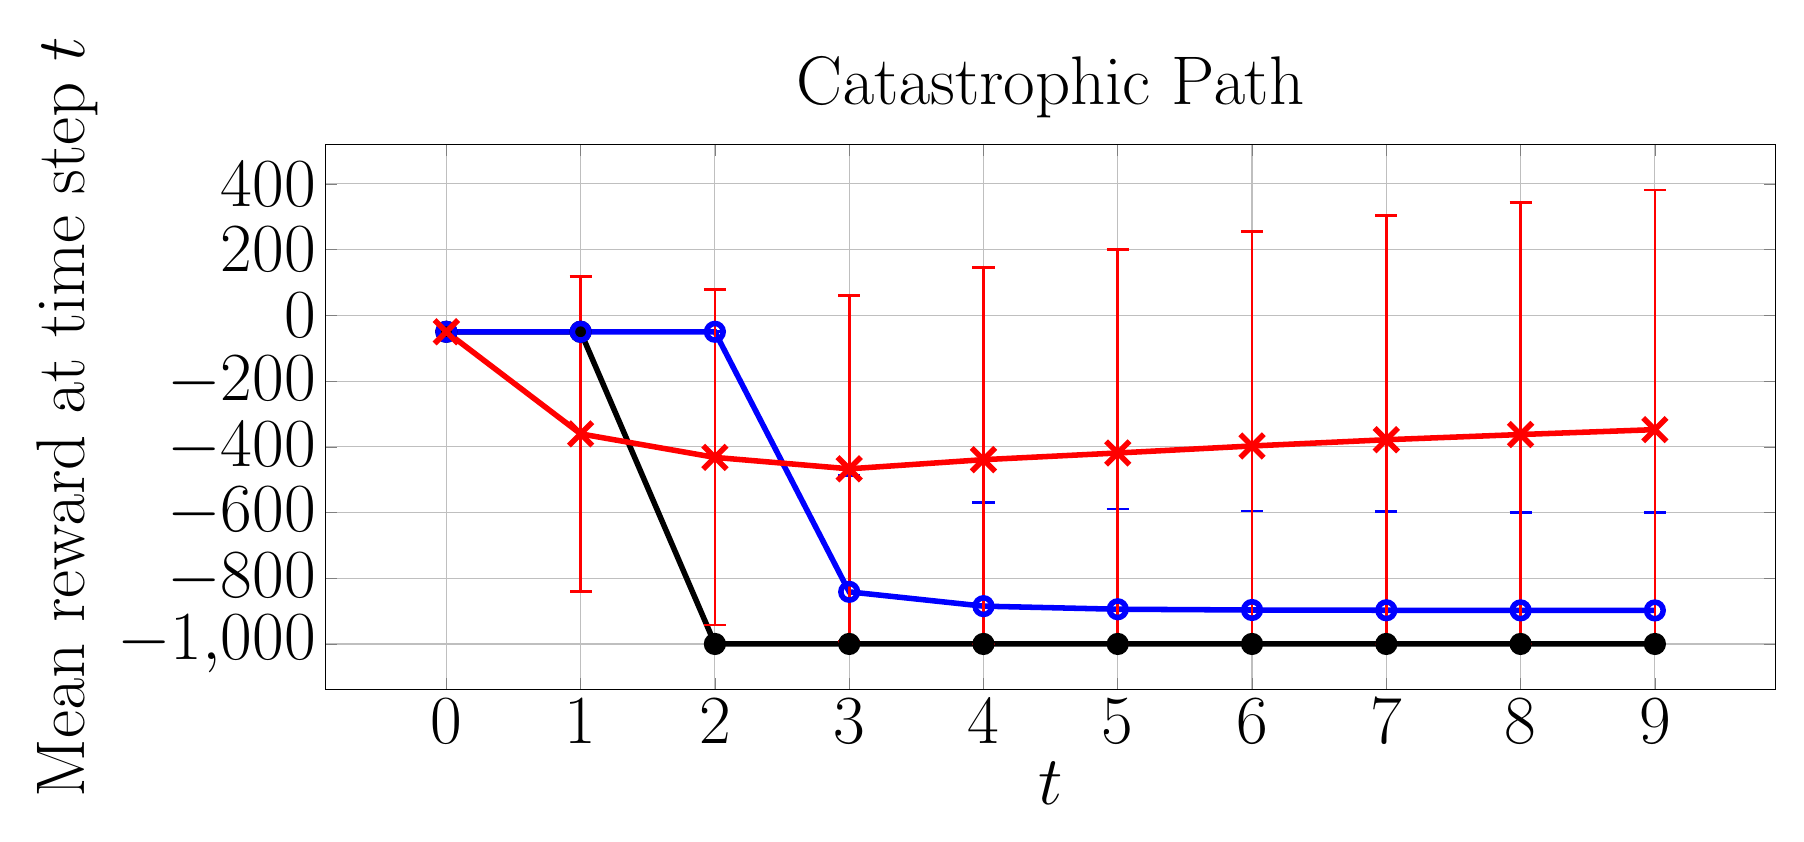
\begin{tikzpicture}
                \begin{axis}[
                    xlabel={$t$},
                    ylabel={Mean reward at time step $t$},
                    title={Catastrophic Path},
                    grid=both,
                    width=20cm, height=8.5cm,
                    every axis/.style={font=\Huge},
                    %
                ]
               \addplot[
                    color=black, %
                    mark=*, %
                    line width=2pt,
                    mark size=3pt,
                ]
                coordinates {
                    (0, -50.0)
                    (1, -50.0)
                    (2, -1000.0)
                    (3, -1000.0)
                    (4, -1000.0)
                    (5, -1000.0)
                    (6, -1000.0)
                    (7, -1000.0)
                    (8, -1000.0)
                    (9, -1000.0)
                };
                %
                %
                \addplot[
                    color=blue, %
                    mark=o, %
                    line width=2pt,
                    mark size=3pt,
                    error bars/.cd,
                    y dir=both, %
                    y explicit, %
                    error bar style={line width=1pt,solid},
                    error mark options={line width=1pt,mark size=4pt,rotate=90}
                ]
                coordinates {
                    (0, -50.0)  +- (0, 0.0)
                    (1, -50.0)  +- (0, 0.0) 
                    (2, -50.0)  +- (0, 0.0) 
                    (3, -841.440725)  += (0, 354.24605512) -= (0, 158.559275)
                    (4, -884.98225)  += (0, 315.37519669) -= (0, 115.01775)
                    (5, -894.330425) += (0, 304.88572805) -= (0, 105.669575)
                    (6, -896.696175) += (0, 301.19954514) -= (0, 103.303825)
                    (7, -897.4635) += (0, 299.61791279) -= (0, 102.5365)
                    (8, -897.77595) += (0, 298.80392585) -= (0, 102.22405)
                    (9, -897.942975) += (0, 298.32920557) -= (0, 102.057025)
                };
                %
                \addplot[
                    color=red, %
                    mark=x, %
                    line width=2pt,
                    mark size=6pt,
                    error bars/.cd,
                    y dir=both, %
                    y explicit, %
                    error bar style={line width=1pt,solid},
                    error mark options={line width=1pt,mark size=4pt,rotate=90}
                ]
            coordinates {
                    (0, -50.0)  +- (0, 0.0)
                    (1, -360.675265)  +- (0, 479.39812699) 
                    (2, -432.27629)  +- (0, 510.38620897) 
                    (3, -467.029545)  += (0, 526.36009628) -= (0, 526.36009628)
                    (4, -439.17429)  += (0, 583.96638919) -= (0, 560.82571)
                    (5, -418.82704) += (0, 618.43027478) -= (0, 581.17296)
                    (6, -397.464895) += (0, 652.67322574) -= (0, 602.535105)
                    (7, -378.49052) += (0, 682.85407033) -= (0, 621.50948)
                    (8, -362.654195) += (0, 707.01412023) -= (0, 637.345805)
                    (9, -347.737935) += (0, 729.29076479) -= (0, 652.262065)
                };
                %
                %
                %
                %
                %
                %
                %
                %
                %
                %
                %
                %
                %
                %
                %
                %
                %
                %
                %
                \end{axis}
            \end{tikzpicture}
         }
    }
    \caption{Average instant reward of CF paths induced by policies on Sepsis.}
    \label{fig: reward sepsis}
\end{figure*}

%
%
%
\subsection{Interval CFMDP Bounds}
%
%
Table \ref{tab:nonzero_probs} presents the mean counterfactual probability bound widths (excluding transitions where the upper bound is $0$) for each MDP, averaged over 20 observed paths. We compare the bounds under counterfactual stability (CS) and monotonicity (M) assumptions, CS alone, and no assumptions. This shows that the assumptions marginally reduce the bound widths, indicating the assumptions tighten the bounds without excluding too many causal models, as intended.
\renewcommand{\arraystretch}{1}

\begin{table}
\centering
\caption{Mean width of counterfactual probability bounds}
\resizebox{0.8\columnwidth}{!}{%
\begin{tabular}{|c|c|c|c|}
\hline
\multirow{2}{*}{\textbf{Environment}} & \multicolumn{3}{c|}{\textbf{Assumptions}} \\ \cline{2-4}
 & \textbf{CS + M} & \textbf{CS} & \textbf{None\tablefootnote{\jl{Equivalent to \citet{li2024probabilities}'s bounds (see Section \ref{sec: equivalence with Li}).}}} \\ \hline
\textbf{GridWorld} ($p=0.9$) & 0.0817 & 0.0977 & 0.100 \\ \hline
\textbf{GridWorld} ($p=0.4$) & 0.552  & 0.638  & 0.646 \\ \hline
\textbf{Sepsis} & 0.138 & 0.140 & 0.140 \\ \hline
\end{tabular}
}
\label{tab:nonzero_probs}
\end{table}


\subsection{Execution Times}
Table \ref{tab: times} compares the average time needed to generate the interval CFMDP vs.\ the Gumbel-max SCM CFMDP for 20 observations.
The GridWorld algorithms were run single-threaded, while the Sepsis experiments were run in parallel.
Generating the interval CFMDP is significantly faster as it uses exact analytical bounds, whereas the Gumbel-max CFMDP requires sampling from the Gumbel distribution to estimate counterfactual transition probabilities. \jl{Since constructing the counterfactual MDP models is the main bottleneck in both approaches, ours is more efficient overall and suitable for larger MDPs.}
\begin{table}
\centering
\caption{Mean execution time to generate CFMDPs}
\resizebox{0.99\columnwidth}{!}{%
\begin{tabular}{|c|c|c|}
\hline
\multirow{2}{*}{\textbf{Environment}} & \multicolumn{2}{c|}{\textbf{Mean Execution Time (s)}} \\ \cline{2-3} 
                                      & \textbf{Interval CFMDP} & \textbf{Gumbel-max CFMDP} \\ \hline
\textbf{GridWorld ($p=0.9$) }                  & 0.261                   & 56.1                      \\ \hline
\textbf{GridWorld ($p=0.4$)  }                 & 0.336                   & 54.5                      \\ \hline
\textbf{Sepsis}                                 & 688                     & 2940                      \\ \hline
\end{tabular}%
}
\label{tab: times}
\end{table}

\section{Conclusion}
In this work, we propose a simple yet effective approach, called SMILE, for graph few-shot learning with fewer tasks. Specifically, we introduce a novel dual-level mixup strategy, including within-task and across-task mixup, for enriching the diversity of nodes within each task and the diversity of tasks. Also, we incorporate the degree-based prior information to learn expressive node embeddings. Theoretically, we prove that SMILE effectively enhances the model's generalization performance. Empirically, we conduct extensive experiments on multiple benchmarks and the results suggest that SMILE significantly outperforms other baselines, including both in-domain and cross-domain few-shot settings.

\section*{Acknowledgment}
This work was supported by the National Key R\&D Program of China under Grant 2022YFB4501400, the National Natural Science Foundation of China (NSFC) grant (62222210, U21B2017 and 62072297). This work was also supported by Shanghai Qi Zhi Institute Innovation Program SQZ202316.  
Cong Guo was supported by Shanghai Jiao Tong University Outstanding Doctoral Graduate Development Scholarship.
The authors express their gratitude to the anonymous reviewers for their insightful feedback, which greatly contributed to improving this work.

\bibliographystyle{IEEEtranS}
\bibliography{paper}

\newpage
% \documentclass[10pt,twocolumn,letterpaper]{article}
\usepackage[rebuttal]{cvpr}

% Include other packages here, before hyperref.
\usepackage{graphicx}
\usepackage{amsmath}
\usepackage{amssymb}
\usepackage{booktabs}
\usepackage{color}
\usepackage{colortbl}
% \usepackage{ulem}
% \useunder{\uline}{\ul}{}
% Import additional packages in the preamble file, before hyperref
%
% --- inline annotations
%
\newcommand{\red}[1]{{\color{red}#1}}
\newcommand{\todo}[1]{{\color{red}#1}}
\newcommand{\TODO}[1]{\textbf{\color{red}[TODO: #1]}}
% --- disable by uncommenting  
% \renewcommand{\TODO}[1]{}
% \renewcommand{\todo}[1]{#1}



\newcommand{\VLM}{LVLM\xspace} 
\newcommand{\ours}{PeKit\xspace}
\newcommand{\yollava}{Yo’LLaVA\xspace}

\newcommand{\thisismy}{This-Is-My-Img\xspace}
\newcommand{\myparagraph}[1]{\noindent\textbf{#1}}
\newcommand{\vdoro}[1]{{\color[rgb]{0.4, 0.18, 0.78} {[V] #1}}}
% --- disable by uncommenting  
% \renewcommand{\TODO}[1]{}
% \renewcommand{\todo}[1]{#1}
\usepackage{slashbox}
% Vectors
\newcommand{\bB}{\mathcal{B}}
\newcommand{\bw}{\mathbf{w}}
\newcommand{\bs}{\mathbf{s}}
\newcommand{\bo}{\mathbf{o}}
\newcommand{\bn}{\mathbf{n}}
\newcommand{\bc}{\mathbf{c}}
\newcommand{\bp}{\mathbf{p}}
\newcommand{\bS}{\mathbf{S}}
\newcommand{\bk}{\mathbf{k}}
\newcommand{\bmu}{\boldsymbol{\mu}}
\newcommand{\bx}{\mathbf{x}}
\newcommand{\bg}{\mathbf{g}}
\newcommand{\be}{\mathbf{e}}
\newcommand{\bX}{\mathbf{X}}
\newcommand{\by}{\mathbf{y}}
\newcommand{\bv}{\mathbf{v}}
\newcommand{\bz}{\mathbf{z}}
\newcommand{\bq}{\mathbf{q}}
\newcommand{\bff}{\mathbf{f}}
\newcommand{\bu}{\mathbf{u}}
\newcommand{\bh}{\mathbf{h}}
\newcommand{\bb}{\mathbf{b}}

\newcommand{\rone}{\textcolor{green}{R1}}
\newcommand{\rtwo}{\textcolor{orange}{R2}}
\newcommand{\rthree}{\textcolor{red}{R3}}
\usepackage{amsmath}
%\usepackage{arydshln}
\DeclareMathOperator{\similarity}{sim}
\DeclareMathOperator{\AvgPool}{AvgPool}

\newcommand{\argmax}{\mathop{\mathrm{argmax}}}     



% If you comment hyperref and then uncomment it, you should delete
% egpaper.aux before re-running latex.  (Or just hit 'q' on the first latex
% run, let it finish, and you should be clear).
\definecolor{cvprblue}{rgb}{0.21,0.49,0.74}
\definecolor{mygray}{gray}{.9}
\usepackage[pagebackref,breaklinks,colorlinks,citecolor=cvprblue]{hyperref}


\newcommand{\re}[2]{\textcolor{#1}{{\bf #2}}}

% Support for easy cross-referencing
\usepackage[capitalize]{cleveref}
\crefname{section}{Sec.}{Secs.}
\Crefname{section}{Section}{Sections}
\Crefname{table}{Table}{Tables}
\crefname{table}{Tab.}{Tabs.}

% If you wish to avoid re-using figure, table, and equation numbers from
% the main paper, please uncomment the following and change the numbers
% appropriately.
%\setcounter{figure}{2}
\setcounter{table}{0}
\renewcommand\thetable{Rb\arabic{table}}
%\setcounter{equation}{2}

% If you wish to avoid re-using reference numbers from the main paper,
% please uncomment the following and change the counter for `enumiv' to
% the number of references you have in the main paper (here, 6).
%\let\oldthebibliography=\thebibliography
%\let\oldendthebibliography=\endthebibliography
%\renewenvironment{thebibliography}[1]{%
%     \oldthebibliography{#1}%
%     \setcounter{enumiv}{6}%
%}{\oldendthebibliography}


%%%%%%%%% PAPER ID  - PLEASE UPDATE
\def\paperID{2514} % *** Enter the Paper ID here
\def\confName{CVPR}
\def\confYear{2025}

\begin{document}

%%%%%%%%% TITLE - PLEASE UPDATE
\title{Category-Level Object Pose Estimation via Causal Learning and Knowledge Distillation}  % **** Enter the paper title here

\maketitle
\thispagestyle{empty}
\appendix

%%%%%%%%% BODY TEXT - ENTER YOUR RESPONSE BELOW
% \section{Introduction}
% \re{red}{R1} \re{blue}{R2} \re{green}{R3}
\noindent
We appreciate reviewers for their valuable feedback, acknowledging the \emph{“clarity and novelty”} (\re{green}{rYxx@R3}) of our core idea, as well as the \emph{“detailed formulation provided”} (\re{blue}{qCQv@R2}). We are encouraged they recognize our approach \emph{“well-organized and easy to follow”} (\re{blue}{R2}, \re{green}{R3}), evaluated with \emph{“extensive experiments”} (\re{green}{R3}), and \emph{“achieving {\bf \emph{SOTA}} performance”} in multiple benchmarks (\re{red}{QHjZ@R1}, \re{blue}{R2}, \re{green}{R3}). We sincerely thank the reviewers for their diligent work and hope our response meets their approval.

\noindent
{\bf $\triangleright$ Responses to individual questions for each reviewer.}

\noindent
\re{red}{@R1 \#w1:} {\bf The Clarity of Paper.}  Thanks for your feedback! Key terms such as \emph{“confounders”} and \emph{“front-door path”} are formally introduced in Sec.3.2 (L201-214), and the causal modeling is illustrated in Fig.2. To improve clarity, we will further enhance the explanation of these key concepts by providing more concrete examples from the task domain and clarifying their roles in the methodology. Additionally, we will confirm that the causal modeling process is presented more intuitively to make it easier to follow.

\noindent
\re{red}{@R1 \#w2:} {\bf The Novelty of Method.} We appreciate your concerns. The key novelty and contribution of our work lies in integrating causal theoretical foundation [36, 37] into COPE models. As Reviewer 3 noted: \emph{“this idea is novel and not straightforward”}. To the best of our knowledge, we are the first to introduce causal modeling to enhance COPE models and achieve significant improvements. Therefore, our work is not simply a combination of existing methods, which involves careful exploration and design that addresses specific challenges mitigating confounding effects.


\noindent
\re{red}{@R1 \#w3:} {\bf Fairness of Comparison.} We would address your comment in two aspects: First, one of the contributions in our work is to explore how to better utilize 3D foundation models to enhance generalization, which is closely related to the overall design of our method, rather than introducing “extra knowledge” that benefits the comparison. Second, 3D foundation model only provides supervision during training, meaning it would not increase any computational burden during inference.
% as shown in \cref{tab:ablation_main} (\#1, \#2).
As for the comparison, we followed the domain consensus to report the metric accuracy.
In response to your suggestions, we have added more terms (\eg encoder type, inference latency) in \cref{tab:ablation_main} for comprehensive comparison. Due to space limitations, detailed comparisons and explanations will be included in revision.

\noindent
\re{blue}{@R2 \#w1:} {\bf Efficacy of Causal Learning.} In fact, as shown in Tab. \textcolor{red}{4}, introducing causal inference can already achieves SOTA results in the rigorous metric of 5°2\emph{cm}, 5°5\emph{cm} and 10°2\emph{cm}, surpassing the baseline by 2.7\%, 1.9\% and 2.8\%. Additionally, as confirmed in \cref{tab:ablation_main}, the front-door adjustment only increases the number of parameters by 10\% (246M \vs 223M), while the running time remains nearly unchanged (33 \vs 35 in FPS).
To ensure a fair comparison, we also replace the front-door module with MLPs that have the same number of parameters (\#3). The results further demonstrate the superior effectiveness of causal learning.


\noindent
\re{blue}{@R2 \#w2:} {\bf Comparison with Feature Concat.} In response to your suggestion, we have concatenated $\mathcal{F}^{ULIP}_{P}$, $\mathcal{F}_{I}$ and $\mathcal{F}_{P}$ for comparison in \cref{tab:ablation_main} (\#4 \vs \#2). The results indicate that the proposed knowledge distillation approach is more effective than feature concatenation.

\noindent
\re{blue}{@R2 \#w3:} {\bf Type of ViT and Additional Comparison.} ViT-S/14 (DINOv2). Following your suggestion, we have added the encoder backbone in \cref{tab:ablation_main}, and included additional results with ResNet18 (\#6). Specifically, our method still outperforms AG-Pose with ResNet18 setting (\#6 \vs \#5), further supporting the efficacy of our approach.

\noindent
\re{green}{@R3 \#w1:} {\bf Reflect of Limitation.} We sincerely acknowledge your valuable feedback! Regarding this limitation, since our method selects PointNet++ as 3D encoder, we hypothesize that when the teacher and student models share similar architectures (\eg, both use PointNet++), the distillation may mislead the student model to focus on feature structure similarity rather than transferring category knowledge. We will add the analysis and detailed difference among three backbones in main text or appendix materials.

\noindent
\re{green}{@R3 \#w2:} {\bf Pose Loss.} L1 loss. We will address it.

\noindent
\re{green}{@R3 \#w4:} {\bf Effect of $N_{s}$.} We speculate that a larger sample size may introduce noise and redundant information that affects key features in causal inference. An appropriate sample size can balance valid and redundant information, prompting the model to focus on learning more representative causal correlations. This will be added in appendix.

\noindent
\re{green}{@R3 \#w5:} {\bf Effect of Sampling.} We have conducted additional experiments with 6 different random seeds, as shown in \cref{tab:inference_samp}. The computed variances $\sigma^{2}$ for metrics demonstrate stable performance across different random seeds, indicating the robustness and reliability of our method.
% Further discussion will be added in revision.

\noindent
\re{blue}{@R2 \#w4}, \re{green}{@R3 \#w3:} {\bf Proofreading.} Thanks for reviewers' reminders and corrections. We will add related works' results and address the caption in revision.
\vspace{-0.3cm}

\begin{table}[htbp]
    \small
    \centering
    \setlength\tabcolsep{4pt}%2pt 列宽
    % \renewcommand\arraystretch{0.9} % 行高
    \begin{tabular}{c|l|c|c|c|c|c}
    % \toprule%[1.2pt]
    \hline
   ID & Method & Encoder & Param.$\downarrow$ & Distill. & 5°2\emph{cm}$\uparrow$  & FPS$\uparrow$\\
    % \midrule%[1pt]
    \hline
    1        &AG-Pose      &  ViT-S/14     &\textbf{223M}          & -    &57.0  &\textbf{35}   \\
    \rowcolor{mygray}
    2         &ours     &ViT-S/14        & \underline{246M}        &Default    &	\textbf{61.5} &\underline{33}   \\
    % \hline
    3        &ours$^*$      &  ViT-S/14      & \underline{246M}          &Default    &59.4 &\underline{33}   \\
    4         &ours     &ViT-S/14        & \underline{246M}        &Concat    &59.8 &31   \\
    \hline
    5         & AG-Pose        & resnet18      & \textbf{220M}          & -   &56.2 &\textbf{35}   \\
    6         & ours        & resnet18      & \underline{243M}          & Default   &\underline{60.3} &\underline{33}   \\
    % \bottomrule%[1.2pt]
    \hline
    \end{tabular}
    \vspace{-0.3cm}
    \caption{Additional results. $*$ denotes replacement of causal module with MLPs of the same number of parameters.
    }
    \label{tab:ablation_main}
\end{table}

\vspace{-0.6cm}

\begin{table}[htbp]
    \small
    \centering
    \setlength\tabcolsep{5pt}%2pt 列宽
    % \renewcommand\arraystretch{0.9} % 行高
    \begin{tabular}{c|cccccc|c}
    % \toprule%[1.2pt]
    \hline
   Seed & 1 & 42 & 500 & 1k & 1w  & 10w& $\sigma^{2}\downarrow$ \\
    % \midrule%[1pt]
    \hline
    5°2\emph{cm}              &  61.4     &61.5         & 61.7    &61.4  &61.3 &61.7&0.03   \\
    5°5\emph{cm}     &67.2        & 67.3        &67.5    &	67.2 &67.1 &67.6&0.04  \\
    % \hline
    % 10°2\emph{cm}              &  78.1      & 78.3          &78.0    &78.0 &78.0  &78.0 &0.01 \\
    % \bottomrule%[1.2pt]
    \hline
    \end{tabular}
    \vspace{-0.2cm}
    \caption{Effect of sampling during inference.
    }
    \label{tab:inference_samp}
\end{table}

% \begin{table}[htbp]
%     \small
%     \centering
%     \setlength\tabcolsep{5pt}%2pt 列宽
%     % \renewcommand\arraystretch{1.2} % 行高
%     \begin{tabular}{c|cccccc|c}
%     \toprule%[1.2pt]
%    $N_{s}$(Infer.) & 6 & 12 & 18 & 24 & 48  & 80& $\sigma^2$ \\
%     % \midrule%[1pt]
%     \hline
%     5°2\emph{cm}$\uparrow$              &  61.1     &\textbf{61.5}         & \underline{61.4}    &60.9  &60.1 &59.9&0.03   \\
%     5°5\emph{cm}$\uparrow$     &66.9        & \textbf{67.4}        &\underline{67.2}    &	66.5 &66.0 &65.8&0.03  \\
%     % \hline
%     10°2\emph{cm}$\uparrow$              &  78.0      & \underline{78.3}          &\textbf{78.5}    &77.8 &77.6  &76.7&0.02 \\
%     \bottomrule%[1.2pt]
%     \end{tabular}
%     \vspace{-0.2cm}
%     \caption{Effect of causal learning and knowledge distillation.
%     }
%     \vspace{-0.2cm}
%     \label{tab:inference_Ns}
% \end{table}



\end{document}



% that's all folks
\end{document}
